%%%% ijcai21-multiauthor.tex

\typeout{IJCAI--21 Multiple authors example}

% These are the instructions for authors for IJCAI-21.

\documentclass{article}
\pdfpagewidth=8.5in
\pdfpageheight=11in
% The file ijcai21.sty is NOT the same than previous years'
\usepackage{ijcai21}

% Use the postscript times font!
\usepackage{times}
\renewcommand*\ttdefault{txtt}
\usepackage{soul}
\usepackage{url}
\usepackage[hidelinks]{hyperref}
\usepackage[utf8]{inputenc}
\usepackage[small]{caption}
\usepackage{graphicx}
\usepackage{amsmath}
\usepackage{booktabs}
\urlstyle{same}

\usepackage{multicol}
\usepackage[final]{changes}
\usepackage{bm}
\usepackage{multirow}
\usepackage{tcolorbox}
\usepackage{rotating}
\usepackage{latexsym,amssymb,amsmath}
\usepackage{makecell}
\usepackage{xspace}
\usepackage{paralist}
\usepackage{wrapfig}
\usepackage{adjustbox}
\usepackage{cite}
%\usepackage{times}
\input{macros-common}
\usepackage{todonotes}

\input{neue_imports}
\newcommand{\pmin}{\rho}

\newcommand{\const}[1]{\mathsf{#1}}

\newcommand{\alphabet}{\Sigma}
\newcommand{\tasks}{\mathcal{A}}
\newcommand{\hidden}{\tau}

\newcommand{\uswn}{SWN\xspace}
\newcommand{\net}{\ensuremath{N}}
\newcommand{\tg}{\ensuremath{G}}
\newcommand{\closed}[1]{\overline{#1}}
\newcommand{\marking}{m}
\newcommand{\enaset}[2]{E_{#2}(#1)}
\newcommand{\fire}[4]{#1\xrightarrow{#2}_{#4}#3}
\newcommand{\probt}[3]{\mathbb{P}_{#2,#3}(#1)}
\newcommand{\prob}[2]{\mathbb{P}_{#2}(#1)}
\newcommand{\rg}[1]{RG(#1)}
\newcommand{\ind}[1]{\textnormal{\texttt{#1}}}
\newcommand{\seq}{\eta}
\newcommand{\run}{\xi}
\newcommand{\trace}{\sigma}
\newcommand{\traces}[1]{\mathit{traces}(#1)}
\newcommand{\ptraces}[2]{\mathit{ptraces}_{#2}(#1)}

\newcommand{\nreach}[3][]{#2 \overset{#1}{\rightsquigarrow} #3}
\newcommand{\runs}[2]{runs_{#2}(#1)}
\newcommand{\seqs}[2]{seqs_{#2}(#1)}
\newcommand{\transp}[1]{#1^\top}
\newcommand{\embed}{\phi}
\newcommand{\trembed}{{\embed^{\text{tr}}}}
\newcommand{\gorgembed}{{\embed^{g}}}


\newcommand{\pa}{\rho_{23}}
\newcommand{\pb}{\rho_{24}}
\newcommand{\pc}{\rho_{55}}
\newcommand{\pd}{\rho_{65}}
\newcommand{\pe}{\rho_{67}}
\newcommand{\pf}{\rho_{57}}

\newcommand{\logtrace}{\trace}
\newcommand{\nonlogtrace}{{\trace'}}


\newcommand{\approptoinn}[2]{\mathrel{\vcenter{
			\offinterlineskip\halign{\hfil$##$\cr
				#1\propto\cr\noalign{\kern2pt}#1\sim\cr\noalign{\kern-2pt}}}}}
\newcommand{\appropto}{\mathpalette\approptoinn\relax}


\newcommand{\unravelled}{unfolded}
\newcommand{\unravelling}{unfolding}
\newcommand{\unravel}{unfold}
\newcommand{\Ind}[1]{\ind{i}_{#1}}


%
%\def\WWITHN{def}
%\ifdefined\WWITHN
%\newcommand{\WCal}[2]{{\mathcal{W}_{#1}^{#2}}}
%\newcommand{\TBf}[2]{{\mathbf{T}_{#1}^{#2}}}
%\else
\newcommand{\TBf}[2]{{\mathbf{G}_{#1}}}
%\fi
\newcommand{\expN}{\closed{\tg_{\rg{\net}}}}

\def\EqualityHolds{itholds}
\ifdefined\EqualityHolds
\newcommand{\probarg}{\tg}
\newcommand{\WCal}[2]{\ptraces{\tg}{#1}}
\else
\newcommand{\probarg}{\expN}
\newcommand{\WCal}[2]{\ptraces{\closed{\tg_{\rg{\net}}}}{#1}}
\fi
\newcommand{\probskip}[1]{\prob{#1}{\probarg}}
\newcommand{\goldenrank}{\mathcal{R}} 



\newlist{myalist}{enumerate*}{1}
\setlist[myalist]{label=\textbf{(\arabic*)}}
\newlist{mylist}{enumerate*}{1}
\setlist[mylist]{label=\textbf{(\roman*)}}
\newlist{alphalist}{enumerate*}{1}
\setlist[alphalist]{label=\textbf{(\alph*)}}

\setlength{\parskip}{0ex}
%\setlength{\parindent}{0ex}
\newlength{\yellownotewidth}
\setlength{\yellownotewidth}{2.5cm}
\newlength{\yellownoteheight}
\setlength{\yellownoteheight}{2.5cm}
%   -   -   -   -   -   -   -   -   -   -   -   -
% Yellow note...
%   -   -   -   -   -   -   -   -   -   -   -   -
\newcommand{\yellownote}[1]{
	\marginpar{
		\vspace{-0.5\yellownoteheight}
		\begin{center}
			\begin{tikzpicture}
			\draw[white,fill=gray!25,opacity=0.75,shift={(-0.125,-0.125)}] 
			(0,0) rectangle (\yellownotewidth,\yellownoteheight);
			\draw[fill=yellow!35] (0,0) rectangle (\yellownotewidth,\yellownoteheight);
			\draw[opacity=0.45,fill=gray!50] (0.7\yellownotewidth,0) -- 
			(0.9\yellownotewidth,0.45) -- (\yellownotewidth,0.4) -- cycle;
			\node[blue,below] at (0.5\yellownotewidth,\yellownoteheight) {
				\begin{minipage}{\yellownotewidth-1em}
				\scriptsize\sf#1
				\end{minipage}
			};
			\end{tikzpicture}
		\end{center}
		\vspace{0.5\yellownoteheight}
	}
}

%   -   -   -   -   -   -   -   -   -   -   -   -
% Resizeable - Yellow note...
%   -   -   -   -   -   -   -   -   -   -   -   -
\newcommand{\resizeableyellownote}[3]{
	\setlength{\yellownotewidth}{#1cm}
	\setlength{\yellownoteheight}{#2cm}
	\marginpar{
		\vspace{-0.5\yellownoteheight}
		\begin{center}
			\begin{tikzpicture}
			\draw[white,fill=gray!25,opacity=0.75,shift={(-0.125,-0.125)}] 
			(0,0) rectangle (\yellownotewidth,\yellownoteheight);
			\draw[fill=yellow!35] (0,0) rectangle (\yellownotewidth,\yellownoteheight);
			\draw[opacity=0.45,fill=gray!50] (0.7\yellownotewidth,0) -- 
			(0.9\yellownotewidth,0.45) -- (\yellownotewidth,0.4) -- cycle;
			\node[blue,below] at (0.5\yellownotewidth,\yellownoteheight) {
				\begin{minipage}{\yellownotewidth-1em}
				\scriptsize\sf#3
				\end{minipage}
			};
			\end{tikzpicture}
		\end{center}
		\vspace{0.5\yellownoteheight}
	}
}



\newcommand{\ADD}[1]{#1}
\usepackage{cancel}
\newcommand\Rcancel[1]{\renewcommand\CancelColor{\color{red}}\cancel{\color{red}#1}}
\newcommand{\colouredcircle}[1]{%
	\tikz{\useasboundingbox (-0.2em,-0.32em) rectangle(0.2em,0.32em);
		\draw[ball color=blue,shading=ball,line width=0.03em] (0,0) circle(0.18em) {#1};}}
\makeatletter
\newcommand\footnoteref[1]{\protected@xdef\@thefnmark{\ref{#1}}\@footnotemark}
\makeatother


\definecolor{ggplotRed}{HTML}{F8766D}
\definecolor{ggplotGreen}{HTML}{7CAE00}
\definecolor{ggplotBlue}{HTML}{00BFC4}
\definecolor{ggplotPurple}{HTML}{C77CFF}


\makeatletter
\g@addto@macro\normalsize{%
\setlength{\abovecaptionskip}{3pt}
\setlength{\belowcaptionskip}{-10pt}
\setlength\abovedisplayskip{3pt}
\setlength\belowdisplayskip{3pt}
\setlength\abovedisplayshortskip{3pt}
\setlength\belowdisplayshortskip{3pt}
}
\makeatother

\usepackage{relsize}
\renewcommand*{\UrlFont}{\ttfamily\smaller\relax}
%\theorempreskip{2pt}
%\theorempostskip{2pt}

\usepackage{cite}

% the following package is optional:
%\usepackage{latexsym}

% Following comment is from ijcai97-submit.tex:
% The preparation of these files was supported by Schlumberger Palo Alto
% Research, AT\&T Bell Laboratories, and Morgan Kaufmann Publishers.
% Shirley Jowell, of Morgan Kaufmann Publishers, and Peter F.
% Patel-Schneider, of AT\&T Bell Laboratories collaborated on their
% preparation.

% These instructions can be modified and used in other conferences as long
% as credit to the authors and supporting agencies is retained, this notice
% is not changed, and further modification or reuse is not restricted.
% Neither Shirley Jowell nor Peter F. Patel-Schneider can be listed as
% contacts for providing assistance without their prior permission.

% To use for other conferences, change references to files and the
% conference appropriate and use other authors, contacts, publishers, and
% organizations.
% Also change the deadline and address for returning papers and the length and
% page charge instructions.
% Put where the files are available in the appropriate places.

\title{Two Approaches to Probabilistic Trace Alignment}

%\author{
%First Author$^1$\footnote{Contact Author}\and
%Second Author$^2$\and
%Third Author$^{2,3}$\And
%Fourth Author$^4$\\
%\affiliations
%$^1$First Affiliation\\
%$^2$Second Affiliation\\
%$^3$Third Affiliation\\
%$^4$Fourth Affiliation\\
%\emails
%\{first, second\}@example.com,
%third@other.example.com,
%fourth@example.com
%}

\makeatletter
\let\@internalcite\cite
\def\cite{\def\citeauthoryear##1##2{##1, ##2}\@internalcite}
\def\shortcite{\def\citeauthoryear##1{##2}\@internalcite}
\def\@biblabel#1{\def\citeauthoryear##1##2{##1, ##2}[#1]\hfill}
\makeatother
% Remove date
\date{\vspace{-5em}} 

\begin{document}

\maketitle

\begin{abstract}
Trace alignment is a prominent problem in AI, whose goal is to detect the trace from a formal 
system that best matches an observation. In the presence of uncertainty, a
formal system can provide only the likelihood of observing a trace. The alignment problem must thus take into account 
the dichotomy between a very similar but unlikely trace, and a very
dissimilar but likely trace. We propose two approaches to probabilistic trace alignment: a precise approach which
needs to be called anew for each alignment test; and an approximate one with a pre-processing step. We also present
specific applications in different AI domains.
\end{abstract}

% !TeX root=../main.tex

\section{Introduction}
\label{introduction}

Trace alignment is a prominent problem in AI, where the goal is to detect the trace, from a formal specification of a system,
which best matches an observed behavior. This has applications in many areas. For example, in Business Process Management (BPM)
one may need to reconstruct the full process from a partially observed trace. Alternatively, if events are not registered immediately,
a log may modify the expected order of events; one should be able to detect and correct these deviations. This is often solved
through a similarity function expressing how close two traces are, according to some criteria.

When the underlying system is vulnerable to uncertainty (e.g., a shipped package may get lost, or a component be defective)
one can no longer express precisely which traces are allowed by the system, but must endow them with a likelihood
of being observed. In this case, the alignment problem must take into account both dimensions: the similarity between the
traces, and the likelihood of being observed. Indeed, it could be that the most similar trace is so unlikely as to be deemed almost
impossible, yielding a suspect alignment. Conversely, the most likely trace may differ too much from the observation to be
meaningful as an alignment. This trade-off must be treated carefully.

We introduce two ranking strategies aiming at finding the most useful alignments. The first one uses a brute force approach that
reuses existing trace aligners like \cite{DBLP:conf/edoc/AdriansyahDA11,LeoniM17}, where the (optimal) ranking
is obtained multiplying the Levenshtein distance between the observed trace and a model trace, by the probability of the
model trace. Although this approach returns the best alignment ranking for an observation, candidate alignments have to be computed
anew for each observation. For models inducing a large number of model traces, this is clearly unfeasible. Our second
strategy tackles this issue by introducing an approximate ranking, where traces are represented as numerical vectors via an embedding.
By exploiting ad-hoc data structures, we retrieve the neighborhood of size $k$ of the observation, by pre-ordering all the collected observations. Instead of analyzing the entire space, we start from the top-$1$ alignment. If the embeddings are
independent of the observation, one embedding can be used to all alignment problems.

We conclude showcasing specific use-cases relevant for AI where our framework can be effectively applied. 
% !TeX root=../main.tex

\section{Preliminaries}
\label{sec:models}
We introduce the basic notions of the formal transition systems and trace alignments that will be used henceforth.

\subsection{Transition Graphs}\label{subsec:ppn}

We consider an abstract model for representing the traces from a process which is based on graphs. These
graphs, which we call \emph{transition graphs} and formalise below, can be further equiped with edge-labels expressing 
the probability of a transition, and hence of a specific trace. The following definition is based on \cite{GartnerFW03}.
\todo{note!! changed the definition of $L$}

\begin{definition} A \emph{(probabilistic) transition graph} (TG) is a tuple $(V,s,t,L,R)$ where:
  \begin{inparaenum}[\itshape (i)]
    \item $V \subset \mathbb{N}$ is a set of \emph{nodes};
    \item $s\in V$ is the \emph{initial node};
    \item $e\in V$ is the \emph{accepting node};
    \item $L: V \to \alphabet$ is the \emph{node labelling function};
    \item $R: V \times V \rightarrow [0,1]$ is a \emph{(probabilistic) transition matrix} indicating, for each pair of nodes, 
    	what is the probability that executing a transition from the first node leads to the second node.
  \end{inparaenum}
Thus $R$ is such that for  every $\ind{i} \in V$, $\sum_{\ind{j}\in V}[R]_{\ind{ij}}=1$.
%
A \emph{weigthed (probabilistic) transition graph} is a pair $(G,\omega)$ where $G$ is a (probabilistic) TG and 
$\omega\in[0,1]$ is its \emph{weight}.
\end{definition}
%
The condition for $R$ ensures that its values can be interpreted as a probability distribution for choosing the next node upon 
executing a transition. $L$ and $R$ determine the probability of reaching a node labeled by $\beta\in\Sigma$ from any node 
labeled $\alpha\in\Sigma$ in $n$ steps by 
$[G.\Lambda^n]_{\alpha\beta}:=L^{-1}(a)R^n L^{-1\top}b$, 
where $L^{-1}$ is seen as a vector (see Example \ref{ex:wheredotiszero}).

\begin{figure}[!t]
	\begin{minipage}{.49\textwidth} 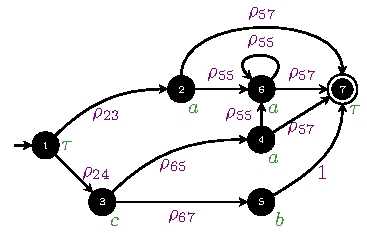
\includegraphics[width=.9\textwidth]{images/closed_example.pdf}
	\caption{A probabilistic TG with abstract weights.}\label{fig:lmc}
\end{minipage}
\end{figure}
%
\figurename~\ref{fig:lmc} shows a TG with the obvious interpretation; an edge from node $\ind{i}$ to node $\ind{j}$ is shown 
(with its weight) only if the transition probability $[\tg.R]_{\ind{i}\ind{j}}$ is positive.
%
A \emph{valid sequence} of the TG $\tg$ is a path $\ind{i}_0\ldots\ind{i}_n$ of nodes in $\tg.V$ from the initial to the 
accepting node using only transitions with positive probability:
\begin{inparaenum}[\it (i)]
\item $\ind{i}_0 = \tg.s$;
\item $\ind{i}_n = \tg.e$;
\item for every $j \in \set{1,\ldots,n}$ we have $[R]_{\ind{i}_{j-1}\ind{i}_{j}} > 0$.
\end{inparaenum}
Runs and model traces of TGs are defined in the obvious manner. We use the same notation to indicate the runs underlying a 
model trace, and the valid sequences underlying a run. The computation of probabilities for runs and traces is defined equivalently.

\subsection{Kernels and Trace Kernels}\label{subsec:katk}
As a foundational basis to compute trace alignments, we adapt similarity measures from the database literature.  Given a set 
of data examples $\mathcal{X}$, a (positive definite) \emph{kernel} function 
$k\colon \mathcal{X}\times \mathcal{X}\to \mathbb{R}$ denotes the similarity of elements in $\mathcal{X}$. If $\mathcal{X}$ is 
the $d$-dimensional Euclidean Space $\mathbb{R}^d$, the simplest kernel function is the inner product $\Braket{\mathbf{x},\mathbf{x}'}=\sum_{1\leq i\leq d}\mathbf{x}_i\mathbf{x}'_i$.
A kernel is said to \emph{perform ideally} \cite{Gartner03} when $k(x,x')=1$ whenever $x$ and $x'$ are the same object (\textit{strong equality}) and $k(x,x')=0$ whenever $x$ and $x'$ are distinct objects (\textit{strong dissimilarity}). A kernel is also said to be \emph{appropriate} when similar elements $x,x'\in\mathcal{X}$ are also close in the feature space. Notice that appropriateness can be only assessed  empirically \cite{Gartner03}.
A positive definite kernel induces a distance metric as:
\begin{equation}\label{eq:dofk}
d_k(\mathbf{x},\mathbf{x}'):=\sqrt{k(\mathbf{x},\mathbf{x})-2k(\mathbf{x},\mathbf{x}')+k(\mathbf{x}',\mathbf{x}')}
\end{equation}
When the kernel of choice is the inner product, the resulting distance is the Euclidean distance $\norm{\mathbf{x}-\mathbf{x}'}{2}$. A normalized vector $\hat{\mathbf{x}}$ is defined as $\mathbf{x}/\norm{\mathbf{x}}{2}$. For a normalized vector we can easily prove that: $\norm{\hat{\mathbf{x}}-\hat{\mathbf{x}}'}{2}^2=2(1-\Braket{\hat{\mathbf{x}},\hat{\mathbf{x}}'})$.

When $\mathcal{X}$ does not represent directly a $d$-dimensional Euclidean space, we can use an \emph{embedding} $\embed\colon\mathcal{X}\to \mathbb{R}^d$ to define a kernel $k_\embed\colon \mathcal{X}\times \mathcal{X}\to\mathbb{R}$ as $k_\embed(x,x'):=\Braket{\embed(x),\embed(x')}$. As a result, $k_\embed(x,x')=k_\embed(x',x)$ for each $x,x'\in\mathcal{X}$.

The literature also provides a kernel representation for strings \cite{LodhiSSCW02,GartnerFW03}, which we can directly employ for our traces. We now provide an intuition describing the desired features of this representation \cite{LodhiSSCW02}. If we associate each dimension in $\mathbb{R}^d$ to a different subtrace $\alpha\beta$ of size $2$ (i.e., $2$-grams\footnote{\label{fn:caveat}For our experiments, we choose to consider only $2$-grams, but any $p$-grams of arbitrary length $p\geq 2$ might be adopted \cite{Gartner03}. An increased size of $p$ improves precision but also incurs in a worse computational complexity, as it requires to consider all the arbitrary subtraces of length $p$ whose constitutive elements occur at any distance from each other within the trace.}), the associated coordinate should represent how frequently and ``compactly'' this subtrace is embedded in the trace $\trace$ of interest. Therefore, we introduce a \emph{decay factor} $\lambda\in[0,1]\subseteq\mathbb{R}$ that, for all $m$ subtraces where $\alpha$ and $\beta$ appear in $\trace$ at the same relative distance $L < |\trace|$, weights the resulting embedding as $\lambda^Lm$.

We need to lift this approach so as to consider all occurrences of subtraces $\alpha\beta$ at every distance between $1$ and $|\trace|-1$. To do so, we proceed in two steps. First, we encode $\trace$ into a ``linear'' transition graph $\tg_\trace$ (\figurename~\ref{fig:taustar}) in the obvious way. %\todo{Tagliare dopo i due punti se necessario.} each node in $G_\sigma.V$  corresponds to an element of the trace labeled correspondingly, and the nodes representing two consecutive elements in the trace are connected with a transition probability of 1 (whereas in all the other cases, the probability is 0).
As a second step, we rely on the matrix operations to calculate a simplified version of the embedding defined in \cite{LodhiSSCW02} as $\trembed_{\alpha\beta}(\trace)=\sum_{1\leq i\leq |\trace|}\lambda^i[(\tg_{\trace}.\Lambda)^i]_{\alpha\beta}$. %\todo{No spazio per spiegare cosa succede...}
%This value can be seen as a reward.
The kernel between two traces corresponds to the sum of the products of such values calculated 2-gram by 2-gram for the two traces.
%, namely it is equal to the \emph{kernel convolution}. %\todo{L'ho provato a scrivere intuitivamente, ma non e' chiaro da dove arrivi questo modo di calcolarlo... deriva dalle formule sopra ma la digressione in mezzo e' lunga. Come possiamo fare per chiarire? L'esempio spiega bene tutto!}
This trace kernel returns strong dissimilarity when the two traces have no shared 2-grams at any arbitrary occurring length, but does not enjoy strong equality (as the similarity of a trace with itself is at least $\lambda^2$ - returned when the trace is a 2-gram).

%
%we can represent it as a TG \cite{Myers1989} $(1,{|\tau|},L_\tau,R_\tau,1)$ having $[L_\tau]_{{\color{green}\alpha}\texttt{\color{blue}i}}=1\Leftrightarrow \tau_{\texttt{\color{blue}i}}={\color{green}\alpha}$ and $[L_\tau]_{{\color{green}\alpha}\texttt{\color{blue}i}}=0$ otherwise, and $\forall i<|\tau|.\; [R_\tau]_{\texttt{\color{blue}i(i+1)}}=1 $ and $[R_\tau]_{\texttt{\color{blue}ij}}=0$ otherwise.
%Exploiting this encoding, we can adopt a simplified version of the embedding defined in \cite{LodhiSSCW02,Raedt} as $\embed_{\mathcal{T}}(\tau)_{{\color{green}\alpha\beta}}=\sum_{1\leq i\leq |\tau|}\lambda^i[(\Lambda_\tau)^i]_{\color{green}\alpha\beta}$.
%Please note that this definition is similar to a transition matrix embedding proposed in \cite{GartnerFW03} via geometric series, that is $\sum_i\lambda^i[R^i]_{\color{green}\alpha\beta}$.

\begin{figure}[!t]
	\centering
	\includegraphics[width=.4\textwidth]{images/taustar.pdf}
	\caption{Graphical representation of the transition graph encoding trace $\const{caba}$.}\label{fig:taustar}
\end{figure}
%
%\begin{example}\label{ex:tracembed}
%	{Let us suppose that we want to align a trace $\tau^*$ to one of the traces from a transition graph: in order to carry out an approximate alignment, we need to transform it to a transition graph first.} A trace $\tau^*=\textup{caba}$ can be graphically represented in Figure \ref{fig:taustar}. The associated TG $T=(\mathtt{\color{blue}1},\mathtt{\color{blue}4},L,R,1)$ has matrices $L$ and $R$  defined as follows:
%	$$L:=\kbordermatrix{
%		& \texttt{\color{blue}1}&\texttt{\color{blue}2}&\texttt{\color{blue}3}&\texttt{\color{blue}4}\\
%		\color{green}a            & 0&\textbf{1}&0&\textbf{1}\\
%		\color{green}b            & 0&0&\textbf{1}&0\\
%		\color{green}c            & \textbf{1}&0&0&0\\
%	}\qquad R:=\kbordermatrix{
%		& \texttt{\color{blue}1}&\texttt{\color{blue}2}&\texttt{\color{blue}3}&\texttt{\color{blue}4}\\
%		\texttt{\color{blue}1}  & 0&\color{red}1&0&0\\
%		\texttt{\color{blue}2}  & 0&0&\color{red}1&0\\
%		\texttt{\color{blue}3}  & 0&0&0&\color{red}1\\
%		\texttt{\color{blue}4}  & 0& 0& 0& 0\\
%	}$$
%We can similarly represent all the traces from the USPN.
%\end{example}

%\begin{example}
%The subtrace \textit{\textbf{\uline{hi}}} is represented in \textit{\textbf{\uline{hi}}deous},   \textit{\uline{\textbf{h}}e\uline{{i}}d\textbf{i}}, and \textit{\uline{{\textbf{h}i}}nd\textbf{i}}, but with different frequencies and subtrace distances. We have $\embed_{\mathcal{T}}(\textit{hideous})_{{\color{green}hi}}=\lambda$,  $\embed_{\mathcal{T}}(\textit{heidi})_{{\color{green}hi}}=\lambda^2+\lambda^4$, and $\embed_{\mathcal{T}}(\textit{hindi})_{{\color{green}hi}}=\lambda+\lambda^4$.
%\end{example}



\begin{table}[t!]
\vspace{+0.5cm}
\caption{Embedding of traces $\const{caba}$, $\const{caa}$ and $\const{cb}$.}\label{tb:embedding}
\vspace{-0.4cm}
\begin{center}
\scalebox{0.45}{
	\begin{tabularx}{\textwidth}{
>{\hsize=.1\hsize}X
>{\hsize=.2\hsize}X
>{\hsize=.1\hsize}X
>{\hsize=.1\hsize}X
>{\hsize=.1\hsize}X
>{\hsize=.1\hsize}X
>{\hsize=.1\hsize}X
>{\hsize=.25\hsize}X
>{\hsize=.2\hsize}X
>{\hsize=.1\hsize}X
}
		\toprule
		& $\const{aa}$    & $\const{ab}$   & $\const{ac}$    & $\const{ba}$   & $\const{bb}$   & $\const{bc}$ & $\const{ca}$ & $\const{cb}$ & $\const{cc}$   \\
		\midrule
		$\const{caba}$ & $\lambda^2$ & $\lambda$ & $0$ & $\lambda$  & $0$  & $0$ & $\lambda+\lambda^3$ & $\lambda^2$ & $0$\\
		%$\const{caaa}$ & $2\lambda+\lambda^2$& $0$ & $0$ & $0$ & $0$ & $0$ & $\lambda+\lambda^2+\lambda^3$ & $0$ & $0$ \\
		$\const{caa}$  & $\lambda$ & $0$ & $0$ & $0$ & $0$ & $0$ & $\lambda+\lambda^2$ & $0$&  $0$\\
		$\const{cb}$   & $0$ & $0$ & $0$ & $0$ & $0$ & $0$ & $0$ & $\lambda$& $0$ \\
		\bottomrule
	\end{tabularx}
}
\vspace{-0.8cm}
\end{center}
\end{table}
\begin{example}\label{ex:wheredotiszero} %\small
Consider tasks $\tasks=\Set{a,b,c}$. The possible 2-grams over $\tasks$ are $\tasks^2=\Set{\const{aa},\const{ab},\const{ac},\const{ba},\const{bb},\const{bc},\const{ca},\const{cb},\const{cc}}$. Table~\ref{tb:embedding} shows the embeddings of some traces. Being a 2-gram, trace $\const{cb}$ has only one nonzero component, namely that corresponding to itself, with $\trembed_{\const{cb}}(\const{cb})=\lambda$. Trace $\const{caa}$ has the 2-gram $\const{ca}$ occurring with length $1$ ($\const{\underline{ca}a}$) and $2$ ($\const{\underline{c}a\underline{a}}$), and the 2-gram $\const{aa}$ with occurring length $1$ ($\const{c\underline{aa}}$). Hence: $\trembed_{\const{ca}}(\const{caa})=\lambda+\lambda^2$ and  $\trembed_{\const{aa}}(\const{caa})=\lambda$.  Similar considerations can be carried out for the other traces in the table.
We now want to compute the similarity between the first trace $\const{caba}$ and the other two traces. To do so, we sum, column by column (that is, 2-gram by 2-gram) the product of the embeddings for each pair of traces. We then get $k_{\trembed}(\const{caba},\const{caa})=\lambda^3+(\lambda+\lambda^3)(\lambda+\lambda^2)$ and $k_{\trembed}(\const{caba},\const{cb})=\lambda^3
$,
%{\footnotesize
%\[
%k_{\trembed}(\const{caba},\const{caaa})=\lambda(\lambda+\lambda^2+\lambda^3)
%~~
%k_{\trembed}(\const{caba},\const{caa})=\lambda(\lambda+\lambda^2)
%~~
%k_{\trembed}(\const{caba},\const{cb})=\lambda(\lambda+\lambda^3)
%\]}
which induces ranking $
k_{\trembed}(\const{caba},\const{caa})>
k_{\trembed}(\const{caba},\const{cb})
$.
\end{example}

\endinput
\subsection{Graph Embedding}\label{ssec:ge}
Graph kernels allow mapping graph data structures to feature spaces (usually an Euclidean space in $\mathbb{R}^n$ for $n\in \mathbb{N}_{>0}$) \cite{Samatova} so to express graph similarity functions that can then be adopted for both classification \cite{TsudaS10} and clustering algorithms. One of the first approaches used in literature involved the definition of topological description vectors \cite{Sidere} for each graph in a graph database, for then defining the graph similarity function as an inner product of their associated vectors. One inconvenience of such a technique is that it is required to perform NP-complete subgraph isomorphisms among a collection of graphs. It has been already proved that the definition of a graph kernel function fully recognizing the structure the graph always boils down to solving such NP-Complete problem \cite{GartnerFW03}, as exact embeddings generable in polynomial can be inferred just for loop-free Direct Acyclic Graphs \cite{BergamiBM20}.


Consequently, most recent literature focused on extracting relevant features of such graphs, that are then used to define a graph similarity function. The most common approach adopted in the kernel to extract such features is called \textit{propositionalization}: we might extract all the possible features (e.g., subsequences), and then define a kernel function based on the occurrence and similarity of these features \cite{Gartner03}.

%\section{LTL over Finite Traces and the Declare Framework}
%\label{sec:preliminaries}
%As a formal basis for specifying crisp (temporal) business constraints, we adopt the customary choice of Linear Temporal Logic over finite traces (\LTLf \cite{DeVa13,DDGM14}). This logic is at the basis of the well-known \declare \cite{PeSV07} constraint-based process modeling language.
%We provide here a gentle introduction to this logic and to the \declare framework.
%
%\subsection{Linear Temporal Logic over Finite Traces}
%
%$\LTLf$ has exactly the same syntax as standard $\LTL$, but, differently from $\LTL$, it interprets formulae over an unbounded, yet finite linear sequence of states. Given an alphabet $\Sigma$ of atomic propositions (in our setting, representing activities), an \LTLf formula $\varphi$ is built by extending propositional logic with temporal operators:
%\[\varphi ::= a \mid \lnot \varphi \mid \varphi_1\lor \varphi_2
% \mid \Next\varphi \mid \varphi_1\Until\varphi_2 \quad \text{ where $a \in \Sigma$.}\]
%
%
%%The semantics of \LTLf is given in terms of \emph{finite traces}
%%denoting finite, \emph{possibly empty}, sequences
%%$\tau=\tau_0,\ldots,\tau_n$ of elements from the alphabet $\Sigma$. The evaluation of a formula is done in a given state (i.e., position) of the trace.
%
%
%The semantics of \LTLf is given in terms of \emph{finite traces} denoting finite, \emph{possibly empty} sequences $\tau=\tup{\tau_0, \ldots, \tau_n}$ of elements of $2^\Sigma$, containing all possible propositional interpretations of the propositional symbols in $\Sigma$. In the context of this paper, consistently with the literature on business process execution traces, we make the simplifying assumption that in each point of the sequence, one and only one element from $\Sigma$ holds. Under this assumption, $\tau$ becomes a total sequence of activity occurrences from $\Sigma$, matching the standard notion of (process) execution trace. We indicate with $\tasks^*$ the set of all traces over $\tasks$. The evaluation of a formula is done in a given state (i.e., position) of the trace, and we use the notation $\tau,i\models \varphi$ to express that $\varphi$ holds in the position $i$ of $\tau$. We also use $\tau \models \varphi$ as a shortcut notation for $\tau,0\models\varphi$. This denotes that $\varphi$ holds over the entire trace $\tau$ starting from the very beginning and, consequently, logically captures the notion of \emph{conformance} of $\tau$ against $\varphi$. We also say that $\varphi$ is \emph{satisfiable} if it admits at least one conforming trace.
%
%%We start by giving an intuitive account of the resulting semantics. In the syntax above, operator $\Next$ denotes the \emph{next state} operator, and $\Next \varphi$ is true if $\varphi$ is true is true now if there exists a next state (i.e., the current state is not at the end of the trace), and in the next state $\varphi$ holds. Operator $\Until$ instead is the \emph{until} operator, and $\varphi_1\Until\varphi_2$ is true if $\varphi_1$ holds now and continues to hold until eventually, in a future state, $\varphi_2$ holds. From the given syntax we can derive the usual boolean operators $\land$ and $\rightarrow$, the two formulae $\true$ and $\false$, as well also additional temporal operators. We consider in particular the following three:
%%\begin{compactitem}[$\bullet$]
%%\item (eventually) $\Diamond \varphi = \true \Until \varphi$ is true if there is a future state where $\varphi$ holds;
%%\item (globally) $\Box \varphi = \neg \Diamond \neg \varphi$ is true if now and in all future sates $\varphi$ holds;
%%\item (weak until) $\varphi_1 \Wntil \varphi_2 = \varphi_1\Until\varphi_2 \lor \Box \varphi_1$ relaxes the until operator by admitting the possibility that $\varphi_2$ never becomes true, in this case by requiring that is true if $\varphi_1$ holds now and in all future states.
%%\end{compactitem}
%% To define the semantics formally, we denote the length of trace $\tau$ as $\length(\tau) =  n+1$.
%
%
%In the syntax above, operator $\Next$ denotes the \emph{next state} operator, and $\Next \varphi$ is true if there exists a next state (i.e., the current state is not at the end of the trace), and in the next state $\varphi$ holds. Operator $\Until$ instead is the \emph{until} operator, and $\varphi_1\Until\varphi_2$ is true if $\varphi_1$ holds now and continues to hold until eventually, in a future state, $\varphi_2$ holds. From these operators, we can derive the usual boolean operators $\land$ and $\rightarrow$, the two formulae $\true$ and $\false$, as well as additional temporal operators. We consider, in particular, the following three:
%\begin{compactitem}[$\bullet$]
%\item (eventually) $\Diamond \varphi = \true \Until \varphi$ is true if there is a future state where $\varphi$ holds;
%\item (globally) $\Box \varphi = \neg \Diamond \neg \varphi$ is true if now and in all future states $\varphi$ holds;
%\item (weak until) $\varphi_1 \Wntil \varphi_2 = \varphi_1\Until\varphi_2 \lor \Box \varphi_1$ relaxes the until operator by admitting the possibility that $\varphi_2$ never becomes true, in this case by requiring that $\varphi_1$ holds now and in all future states.
%\end{compactitem}
%%We write $\tau \models \varphi$ as a shortcut notation for $\tau,0\models \varphi$, and say that formula $\varphi$ is \emph{satisfiable}, if there exists a trace $\tau$ such that $\tau \models \varphi$.
%
%\begin{example}
%The $\LTLf$ formula $\Box(\activity{accept} \rightarrow \Diamond\activity{pay})$ models that, whenever an order is accepted, then it is eventually paid. The structure of the formula follows what is called \emph{response template} in \declare.
%\end{example}
%
%%Every $\LTLf$ formula $\varphi$ can be translated into a corresponding standard finite-state automaton $\aut_\varphi$ that accepts all and only those finite traces that satisfy $\varphi$ \cite{DeVa13,DDGM14}. Although the complexity of reasoning with $\LTLf$ is the same as that of $\LTL$, finite-state automata are much easier to manipulate in comparison with B\"uchi automata, which are necessary when formulae are interpreted over infinite traces.
%
%\subsection{Declare}
%\input{declare-templates}
%\declare\ \cite{PeSV07} is a declarative process modeling language based on \LTLf. More specifically, a \declare model fixes a set of activities, and a set of constraints over such activities, formalized using \LTLf formulae. The overall model is then formalized as the conjunction of the \LTLf formulae of its constraints.
%
%Among all possible \LTLf formulae, \declare selects some pre-defined patterns. Each pattern is represented as a \declare template, i.e., a formula with placeholders to be substituted by concrete activities to obtain a constraint. Constraints and templates have a graphical representation; Table~\ref{tab:constraints} lists the \declare templates used in this paper. A \declare model is then graphically represented by showing its activities, and the application of templates to such activities (which indicates how the template placeholders have to be substituted to obtain the corresponding constraint).
%
%%Automata-based techniques for $\LTLf$ have been adopted to tackle fundamental tasks within the lifecycle of \declare processes, such as consistency checking \cite{PeSV07,MPVC11}, enactment and monitoring \cite{PeSV07,MMWV11,DDGM14}, and discovery support \cite{MaCV12}.
%
%
%
%
%\begin{example}
%\label{ex:inconsistency}
%Consider the following \declare model, constituting a (failed) attempt of capturing a fragment of an order-to-shipment process:
%
%\begin{center}
%  \resizebox{3.2cm}{!}{
%        \begin{tikzpicture}
%        \node[task] (accept) {\accept};
%        \node[task,right=of accept] (reject) {\reject};
%        \node[left=0mm of accept,taskfg] {1..*};
%        \node[right=0mm of reject,taskfg] {1..*};
%        \draw[notcoexistence] (accept) -- (reject);
%    \end{tikzpicture}
%  }
%\end{center}
%
%The model indicates that there are two activities to accept or reject an order, that these two activities are mutually exclusive, and that both of them have to be executed.
%%  \begin{wrapfigure}[13]{l}{42mm}
%%  \end{wrapfigure}
%These constraints are obviously contradictory and, in fact, the model is inconsistent, since its \LTLf formula
%$
%\Diamond \accept \land \Diamond \reject \land \neg (\Diamond \accept \land \Diamond \reject)
%$
%is unsatisfiable.
%\end{example}
%
%
%
%\endinput
%
%\smallskip\noindent\textbf{\declare} is a constraint-based process modeling language based on \LTLf. Differently from imperative process modeling languages,
%\declare models a process by fixing a set of activities, and defining a set of
%\emph{temporal constraints} over them, accepting every execution trace that satisfies all constraints.
%Constraints are specified via pre-defined \LTLf templates, which come with a corresponding
%graphical representation (see Table~\ref{tab:constraints} for the \declare patterns we use in this paper).
%For the sake of generality, in this paper we consider arbitrary \LTLf formulae as constraints. However, in the examples we consider formulae whose templates can be represented graphically in \declare.
%
%
%
%Automata-based techniques for $\LTLf$ have been adopted in \declare to tackle fundamental tasks within the lifecycle of Declare processes, such as consistency checking \cite{PeSV07,MPVC11}, enactment and monitoring \cite{PeSV07,MMWV11,DDGM14}, and discovery support \cite{MaCV12}.

% !TeX root=../main.tex

\section{Probabilistic Trace Alignment Pipeline}
We now provide a technique for computing probabilistic trace alignments. Our approach takes as input
\begin{inparaenum}[\it (i)]
\item a reference model represented as a TG $\tg$,
\item a minimum, positive probability threshold $\pmin \in (0,1]$
\item a trace $\trace$ of interest,
\end{inparaenum}
and returns a ranking over all the $\net$-traces having a probability at least $\pmin$, based on a combination of their probabilities
(probabilistic component) and their distance to $\trace$ (alignment component).


\subsection{Computation pipeline}
We follow the pipeline shown in \figurename~\ref{fig:pipe} and described next.
%
\begin{figure}[!t]
	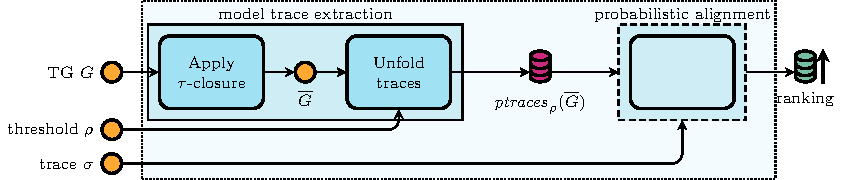
\includegraphics[width=\columnwidth]{images/pipelineShort}
	\caption{Pipeline to assess the probabilistic trace alignment.}\label{fig:pipe}
\end{figure}
%
%
%In step 1, the reachability graph $\rg{\net}$ of $\net$ is constructed.
%%
%In step 2,  $\rg{\net}$ is converted into a corresponding transition graph $\tg_{\rg{\net}}$ that preserves model traces and their
%probabilities. We omit the details of this conversion, due to lack of space and the fact that it employs well-known techniques used
%to \emph{shift labels} from transitions to states while preserving the behavior encoded by a transition system.
%\figurename~\ref{fig:orig} shows the result of this conversion when applied to the reachability graph in \figurename~\ref{fig:rg}.
%
The original TG $\tg$ is processed through a \emph{$\hidden$-closure} that compiles away all invisible transitions, resulting in
a new TG $\closed{\tg}$ using $\hidden$ labels only in the initial and accepting states, without modifying the
model traces or their probabilities. We omit the details, which rely on well-known automata-based techniques for removing
$\epsilon$-moves. The only observation is that, to preserve probabilities, we assume that the TG has no $\tau$ loops with
positive probability. In other words, we assume that all possible movements are observable.
The TG in \figurename~\ref{fig:lmc} already has this shape.

The next step unfolds the TG $\closed{\tg}$ to collect all the traces with probability at least $\pmin$. For this, we rely on a key
property of loops. Since the probability of a path is the product of the probabilities of the transitions, a loop can only have
probability 1 if all its transitions have probability 1 themselves. Assuming no periodic behavior appears, an execution of a
loop must decrease the probability. Thus, all valid sequences with a resulting probability of at least $\pmin$ can be enumerated.
These sequences are merged by trace, summing up their probabilities, thus obtaining the set $\ptraces{\closed{\tg}}{\pmin}$
of all the distinct traces having a probability at least $\pmin$. The closure operation ensures that the notion of model trace collapses to
that of run modulo removing the initial and the final $\tau$ labels attached to the initial and accepting nodes.

The last step ranks the model traces considering their probabilities and the similarity with the input trace $\trace$. In
\figurename~\ref{fig:pipe}, this is shown as a black-box. We implement this last step in two alternative ways: one
computationally demanding but guaranteeing an optimal ranking, the other more efficient but yielding approximate ranking without
optimality guarantees.

\endinput

%%%%%%%%%%%%%%%%%%%%
%%%%%%%%%%%%%%%%%%%%
%%% END INPUT
%%%%%%%%%%%%%%%%%%%%
%%%%%%%%%%%%%%%%%%%%

%
We can show that the TG obtained in Definition \ref{def:transf} preserves the same set of probabilistic traces associated by the reachability graph. The proof is omitted due to the lack of space.

\begin{example}
\figurename~\ref{fig:lmc} shows the TG obtained from the reachability graph in \figurename~\ref{fig:rg}. Nodes are labeled with the firing
transition labels (in green), and edges preserve the probabilistic information from the reachability graph (in red). Intuitively, when a
new initial node \textit{\textbf{i}} is inserted, we preserve all the initial probabilistic choices that a transition is fired from an initial
marking $M$, while the intermediate edges inherit the probabilistic choice of the firing transition from the subsequent choices. When
a new final node \textit{\textbf{f}} is added, such edges always have probability $1$, and thus do not interfere with the
initial traces' probability.
\end{example}

\subsection{$\tau$-closure}\label{sec:clos}
The $\tau$-closure process has two main purposes: first, reduce the size of the previously generated TG by removing all
$\tau$-labeled nodes \texttt{\color{blue}w} and preserving the connection between  the nodes \texttt{\color{blue}u}
from its ingoing edges   $\texttt{\color{blue}u}\xrightarrow{\color{violet}\rho}\texttt{\color{blue}w}$ with the nodes \texttt{\color{blue}v} from its ingoing edges   $\texttt{\color{blue}w}\xrightarrow{\color{violet}\rho'}\texttt{\color{blue}v}$ by establishing new edges $\texttt{\color{blue}u}\xrightarrow{\color{violet}\rho\rho'}\texttt{\color{blue}v}$. $\tau$-labeled initial (or accepting) nodes are removed iff they have only one outgoing (ingoing) edge with probability $1$.

\begin{example}\todo{Is it now ok?}
	The $\tau$-closure removes the non-initial and non-accepting nodes within an automaton, while preserving the probabilistic trace equivalence of the two automata. Let us suppose to apply the $\tau$-closure to the automata in \figurename~\ref{fig:orig}: node \texttt{\color{blue}10} is removed alongside its associated edges, and new edges $\texttt{\color{blue}3}\xrightarrow{\color{violet}\rho_{65}}\texttt{\color{blue}4}$ and $\texttt{\color{blue}3}\xrightarrow{\color{violet}\rho_{6f}}\texttt{\color{blue}5}$ are introduced. The resulting TG $P$ is represented with the same graphical depiction \figurename~\ref{fig:closed}.
\end{example}
%
Consequently, it is always possible to minimize a TG  via $\tau$-closure, so that the only nodes labeled as $\tau$
are the source and the target nodes and the set of weighted traces is preserved. From now on, we consider only minimized TGs.

\subsection{Unfolder}\label{sec:unrav}
%Being that both the graph isomorphism problem is NP-Complete and the
Since TGs are fully characterized by the set of the probabilistic traces that they generate,  we say that two TGs are
(probabilistic-trace) equivalent iff they share the same set of weighted traces. In particular, we denote as $\mathcal{W}_p^n(P)$ the set of all the weighted traces in $P$ having at least probability $p$ and maximum length $n$. Under these assumptions, the probabilistic trace equivalence is deterministic.

\begin{example}
	The set $\mathcal{W}_0^{\aleph_0}(P^*)$ of weighted traces of the TG in \figurename~\ref{fig:orig} is
%	The TG in \figurename~\ref{fig:orig} has the following set $\mathcal{W}_0^{\aleph_0}(P^*)$ of weighted traces:
$$\set{\braket{\underbrace{\color{green}a\dots a}_{n},{\color{violet}\pa\pc^n\pf}}|n\in \mathbb{N}_{>0}}\cup \set{\braket{{\color{green}c}\underbrace{\color{green}a\dots a}_{n},{\color{violet}\pb\pd\pc^n\pf}}|n\in \mathbb{N}_{>0}}\cup\{\braket{{\color{green}cb},{\color{violet}\pb\pe}}\}$$
After the $\tau$-closure process, $\mathcal{W}_0^{\aleph_0}(P^*)=\mathcal{W}_0^{\aleph_0}(P)$, so the two TGs are (probabilistic-trace) equivalent.
\end{example}

% !TeX root=../main.tex

\subsection{Alignment Strategy}\label{subsec:as}
When aligning a log trace with a TG, retrieving the model trace maximizing the combined provision of minimum trace alignment cost 
and maximum model trace probability does not suffice.
Hence, we find the best $k$ alignments among all the distinct \unravelled\ model traces in $\ptraces{\tg}{\pmin}$. This is
known as the $k$-nearest neighbors ($k$NN) problem of finding the $k$ nearest data points to a \textit{query} $x$ from a set 
$\mathcal{X}$ of \textit{data points} w.r.t.\ a given distance function $d_k$. Through ad-hoc data structures, such as VP-Trees 
and KD-Trees, %VP-Trees \cite{Fu2000} \cite{Maneewongvatana99}, and M-Trees \cite{Ciaccia},
we can retrieve the $k$-neighborhood of $x$ in $\mathcal{X}$ by pre-ordering (\textit{indexing}) $\mathcal{X}$ w.r.t.\ $d_k$ 
and searching from the top-$1$ alignment.
%
To align a trace $\logtrace$ over the \unravelled\ traces $\ptraces{\tg}{\pmin}$,
the $k$-Nearest Neighbors describe the best $k$ alignments for $\logtrace$. We discuss two strategies to obtain these
alignments.

\noindent
\textbf{Optimal-Ranking Trace Aligner.}
One approach is to reuse existing trace aligners; e.g., \cite{DBLP:conf/edoc/AdriansyahDA11,LeoniM17} over the Levenshtein 
distance.
Using decision theory \cite{dectheor}, we express the ranking score as the product 
$\probskip{\nonlogtrace} d(\logtrace,\nonlogtrace)$, taking into account the cost of the alignment (the distance between 
the model trace and the trace to be aligned) and the probability of the model trace.

To represent the same intuition of a weighted distance as a ranking function, we transform it into a
similarity function returning $1$ when $\nonlogtrace=\logtrace$ and $\probskip{\logtrace}=1$ hold. We express $d$ as
a normalized similarity score $s_d(\logtrace,\nonlogtrace):=\frac{1}{\frac{1}{c}d(\logtrace,\nonlogtrace)+1}$, where  
$c\in\mathbb{N}_{\neq0}$ is a constant. The maximum similarity is reached when the distance is $0$ and the similarity decreases 
as the distance increases. 
 The golden ranking function producing the optimal ranking is 
 $\goldenrank(\logtrace,\nonlogtrace)=\probskip{\nonlogtrace} \probskip{\logtrace} s_d(\logtrace,\nonlogtrace)$;
${\max\arg}_{\nonlogtrace\in \WCal{\pmin}{n}} \goldenrank(\logtrace,{\nonlogtrace})$ yields the best optimal-ranking trace 
alignment for a log trace $\logtrace$, where $\goldenrank$ must be computed anew for each possible $\logtrace$. 
\ADD{We can represent each trace as a point  $(\mathbb{P}_N(\sigma)\mathbb{P}_N(\sigma'),\; s_d(\sigma,\sigma'))$ in the 
2-dimensional similarity/probability space of coordinates $(p,s)$, reducing the trace finding problem to maximising the product 
$p\cdot s\equiv \mathbb{P}_N(\sigma)\mathbb{P}_N(\sigma')\cdot s_d(\sigma,\sigma')$ (Figure \ref{fig:sps}).}
%
\begin{figure}[!t]
	\centering
	\subfloat{\label{fig:spp}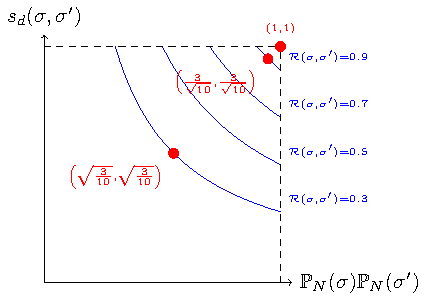
\includegraphics[width=.35\textwidth]{images/original_space.pdf}}\qquad
	\subfloat{\label{fig:knnspace}\includegraphics[width=.33\textwidth]{images/transformed_space.pdf}}\\
	\caption{Two characterizations of probabilistic trace alignment; the similarity/probability space above, and the transformed
	$k$NN space below. The best possible match is shown in red in both spaces.}\label{fig:sps}
\end{figure}


\begin{table}[!t]
\centering
\caption{Golden ranking of $\ptraces{\closed{\tg}}{0}$ with maximum length $4$, where $\logtrace=\const{caba}$ and $c=5$.}\label{tab:expected}
\resizebox{.45\textwidth}{!}{\begin{tabular}{lc|ll|c}
	\toprule
	
	{$\nonlogtrace$} &
	{$d(\sigma',\sigma)$} &
	$( \mathbb{P}_N(\sigma')$ &  $,\,s_d(\sigma',\sigma)) $ &
	{$\approx s_d(\sigma,\sigma^*)\cdot w_\sigma$} \\
	
	
	\midrule
	$\const{a}$  & $3$ & $0.4$ & $\;\; 0.6250$  & $0.2500$\\
	$\const{aa}$  & $2$ & $0.2$ & $\;\; 0.7142$ & $0.1428$\\
	$\const{aaa}$  & $2$ & $0.1$ & $\;\; 0.7142$ & $0.0714$ \\
	$\const{ca}$  & $2$ & $0.07$ & $\;\; 0.7142$ & $0.0500$\\
	$\const{cb}$  & $2$ & $0.06$ & $\;\; 0.7142$ & $0.0428$ \\
	$\const{aaaa}$  & $3$ & $0.05$ & $\;\; 0.7142$ & $0.0357$ \\
	$\const{caa}$  & $1$ & $0.035$ & $\;\; 0.8333$ & $0.0292$ \\
	$\const{caaa}$  & $1$  & $0.0175$ & $\;\; 0.8333$ & $0.0145$ \\
	\bottomrule
\end{tabular}}
\end{table}
\begin{example}\label{ex:rankingTaus}
Consider the TG $\closed{\tg}$ in \figurename~\ref{fig:lmc} with probabilities
$\pa=0.8$, $\pb=0.2$, $\pc=\pf=0.5$, $\pd=0.7$, and $\pe=0.3$. The traces with maximum length $4$ are:
%$$\begin{aligned}
%\ptraces{\expN}{0}_{|\nonlogtrace|\leq 4}=
$\{\braket{\const{a},0.4},\braket{\const{aa},0.2}$, $\braket{\const{aaa},0.1}$, $\braket{\const{ca},0.07}$, 
$\braket{\const{cb},0.06}$,
$\braket{\const{aaaa},0.05},\braket{\const{caa},0.035},\braket{\const{caaa},0.0175}\}$. 
Table \ref{tab:expected} represents their alignment raking with  $\nonlogtrace=\textup{caba}$.  Although $\const{caa}$ and 
$\const{caaa}$ are the most similar to $\const{caba}$, their associated probability  is rather low, so traces with 
higher probability but lower similarity score are preferred (e.g., $\const{a}$ and $\const{aa}$).
\end{example}
%
\ADD{Since users might still prefer the most similar ones to the ones maximizing both probability and similarity, we 
return the best $k$ solutions.
We reduce the problem to $k$NN over the Euclidean Space through a transformation $t$ such that the distance of the 
transformed point $t(p,s)$ from  the origin $\vec{0}$ is $\sfrac{1}{ps}$. This preserves the score from the golden ranking 
and maps the points maximizing $ps$ nearer to the origin. We choose}
$t(p,s):=\left(\frac{1}{s\sqrt{p^2+s^2}},\; \frac{1}{p\sqrt{p^2+s^2}}\right)$. 
Our search always starts from the origin, and hence finds the best candidates first.
	
%
\begin{example}
\ADD{Figure \ref{fig:sps} (above) shows a family of hyperbolae $ps$ with all the alignments having 
$\mathcal{R}(\sigma,\sigma')=ps$. Point $\color{red}(1,1)$ is the best possible trace match, i.e., a trace 
$\nonlogtrace\in\ptraces{G}{0}$ with $\nonlogtrace=\logtrace$ and $\mathbb{P}_G(\nonlogtrace)\mathbb{P}_G(\logtrace)=1$.
%		
Figure \ref{fig:knnspace} (below) shows that the embedding moves the points of the hyperbola $ps$ to a circumference $x^2+y^2=\sfrac{1}{(ps)^2}$ describing a locus of the points equidistant as $\sfrac{1}{ps}$ from the origin of the axes $(0,0)$.}
\end{example}
%
The transformation required for running the $k$NN algorithm preserves the ranking induced by $\mathcal{R}$.

\begin{lemma}
The set of points having the product $ps$ at least $k\in[0,1]$ corresponds to the set of $t$-transformed points with distance 
at least $1/k$ from the origin.
\end{lemma}
%
%\begin{proof} 
%\todo{may be removed if needed}
%Ignoring the irrelevant traces for $ps= 0$, we have:
%	\[
%	ps\geq k\Leftrightarrow \frac{1}{ps}=
%	{ \frac{\sqrt{p^2+s^2}}{ps\sqrt{p^2+s^2}}= \left\|t(p,s)-\vec{0}\right\|_2\leq\frac{1}{k} }\\
%	%&{\Leftrightarrow \sqrt{\frac{p^2+s^2}{p^2s^2(p^2+s^2)}}\leq\frac{1}{k}} \\
%%	&{\Leftrightarrow \sqrt{\frac{p^2}{p^2s^2(p^2+s^2)}+\frac{s^2}{p^2s^2(p^2+s^2)}}\leq\frac{1}{k}} \\
%%	&{\Leftrightarrow \sqrt{\frac{1}{s^2(p^2+s^2)}+\frac{1}{p^2(p^2+s^2)}}\leq\frac{1}{k}} \\
%%	&{\Leftrightarrow \left\|{\biggr({\frac{1}{s\sqrt{p^2+s^2}},\frac{1}{p\sqrt{p^2+s^2}}\biggr)}-\vec{0}}\right\|_2\leq\frac{1}{k}} \\
%\]
%\end{proof}
	
\noindent
\textbf{Approximate-Ranking Trace Embedder.}\label{subsec:ate}
Ranking optimality comes at the cost of a brute-force recomputation of $\goldenrank$ for each trace $\logtrace$ to align.
Since each embedding $\phi$ entails an associated similarity metric $k_\phi$ (\S\ref{subsec:katk}) and hence an associated
distance $d_{k_\phi}$ (Equation \ref{eq:dofk}), we can compute the embeddings for all the \unravelled\ traces
before the top-$k$ search ensuring that they are independent of the trace to align, avoiding the brute-force cost. 
This computational gain comes with a loss in precision; the generation of precise embeddings for graph data with loops is 
NP-complete \cite{GartnerFW03} and, in its approximated version, is unable to accurately represent data using low-dimensional 
vectors \cite{Seshadhri5631}. Our proposed embedding ($\gorgembed$) is thus weakly-ideal (\S\ref{subsec:katk}).

$\gorgembed$ is a variant of the embedding $\trembed$ from \cite{LodhiSSCW02}, which addresses some of its shortcomings.
Indeed, $\trembed$
\begin{alphalist}
 \item is not weakly-ideal, so we cannot numerically assess if two embeddings represent equivalent traces 
 (Example \ref{ex:wheredotiszero});
 \item does not characterize $\tau$-moves, so the probabilities of the initial and final $\tau$-moves are not preserved; and
 \item is affected by numerical errors from finite arithmetics: longer traces $\nonlogtrace$ generated from skewed probability 
 	distributions $G.\Lambda^i$ yield greater truncation errors, as smaller $\lambda^i$ components for bigger 
 	$i<|\nonlogtrace|$ are ignored, preventing a complete numerical vector characterization of  $\nonlogtrace$ in practice.
\end{alphalist}
%
To overcome these shortcomings we 
\begin{alphalist} 
\item propose a weakly-ideal embedding, which also 
\item exploits an $\omega$ factor for preserving probabilities from and to $\tau$ transitions, and 
\item mitigate the numerical truncation errors induced by trace length and probability distribution skewness through two 
sub-embedding strategies, $\epsilon^x$ and $\nu^x$. The former descends from $\trembed$ and the latter approximates 
the trace similarity through label frequencies.
\end{alphalist}

Since a trace embedding for $\nonlogtrace$ representing the transitions in $\closed{\tg}.\Lambda$ requires an intermediate 
TG representation, each $\nonlogtrace$ is mapped to a transition graph $\tg_\nonlogtrace$.
%
\begin{definition}[trace projection]
Let $\closed{G}=(V,s,t,L,R)$ be a $\tau$-closed TG, and $\pmin\in(0,1]$. The $\closed{G}$ \emph{projection} over the trace 
$\nonlogtrace$ is the weighted TG $(\closed{G}_\nonlogtrace,\omega)$, where $\closed{G}_\nonlogtrace$ is the TG 
$(V_\nonlogtrace,s,t,L_\nonlogtrace,R_\nonlogtrace)$ where
$V_\nonlogtrace$ contains the nodes generating $\nonlogtrace$ from $\closed{G}$	
	(i.e., $\bigcup_{\xi\in\runs{\nonlogtrace}{\closed{G}}}\seqs{\xi}{ \closed{G}}$) and
$L_\nonlogtrace$ and $R_\nonlogtrace$ are the restrictions of $L$ and $R$ to $V_\nonlogtrace$; and
$$\omega := 1-\prod_{\xi\in\runs{\sigma}{\closed{G}},\eta\in\seqs{\xi}{\closed{G}}}\Big(1-(\textit{ifte}([L]_{\tau\eta_1},[R]_{\eta_1\eta_2})\textit{ifte}([L]_{\tau t_n},[R]_{t_{n-1} t_n})\Big),$$
	where $\textit{ifte}(x,y):=x(y-1)+1$ returns $y$ if $x=1$ and $1$ otherwise. We denote the set of all the $\closed{G}_\nonlogtrace$ as $\TBf{\pmin}{4}(\closed{G})$.\todo{need to understand this}
%\dots
%		
%		\dots we generate a set $\TBf{\pmin}{n}(\closed{G})$ of projected TGs $P$ for each trace in $\WCal{\pmin}{n}(P)$ as follows: for each weighted trace $\braket{\nonlogtrace,\probskip{\nonlogtrace}}\in\WCal{\pmin}{n}(P)$ generated from a path $\pi_\nonlogtrace=s\to n_2\rightsquigarrow n_m\to t$ over $R$, we generate a TG $P_\nonlogtrace=(s',t',L_\nonlogtrace,R_\nonlogtrace,\omega')$, where \begin{inparaenum}[\it (i)]
%			\item $s'=s$ if $\textit{label}(s)\neq \tau$ and $t'=n_2$ otherwise,
%			\item $t'=t$ if $\textit{label}(t)\neq \tau$ and $t'=n_m$ otherwise,
%			\item $L_\nonlogtrace$ (and $R_\nonlogtrace$) is the submatrix of $L$ (and $R$) over the non-$\tau$ labeled notes in $\pi_\nonlogtrace$ and the labels from $\nonlogtrace$,
%			\item $\omega'$ is initialized by $\omega$ and then multiplied by $[R]_{s,n_2}$ (and also $[R]_{n_m,t}$) if $\textit{label}(s)=\tau$ (and  $\textit{label}(t)=\tau$).
%		\end{inparaenum}
\end{definition}
%	
\begin{table}[!t]
	\caption{Projections of $\tg$ over traces of length $4$.}\label{tab:proj}
	\centering
	\resizebox{.28\textwidth}{!}{\begin{tabular}{>{\centering\arraybackslash} m{1cm}| >{\centering\arraybackslash} m{4cm} >{\centering\arraybackslash} m{1cm} >{\centering\arraybackslash} m{1cm} }
			\toprule
			$\nonlogtrace$&$G_\nonlogtrace$&$l$&$\omega$\\
			\midrule
			$\const{a}$ & \includegraphics{images/trace_a} & $1$ & $\color{violet}\pa\pf$\\
			$\const{cb}$ & \includegraphics{images/trace_cb} & $2$ & $\color{violet}\pb$\\
			$\const{aaa}$ & \includegraphics{images/trace_a_loop} & $3$ & $\color{violet}\pa\pf$\\
			$\const{caa}$ & \includegraphics{images/trace_caa} & $3$ & $\color{violet}\pb\pf$\\
%			\bottomrule
%	\end{tabular}}\qquad 	
%	\resizebox{.3\textwidth}{!}{\begin{tabular}{>{\centering\arraybackslash} m{1cm}| >{\centering\arraybackslash} m{4cm} >{\centering\arraybackslash} m{1cm} >{\centering\arraybackslash} m{1cm} }
%	\toprule
%	$\nonlogtrace$&$G_\nonlogtrace$&$l$&$\omega$\\
%	\midrule
	$\const{aa}$ & \includegraphics{images/trace_aa} & $2$ & $\color{violet}\pa\pf$\\
	$\const{ca}$ & \includegraphics{images/trace_ca} & $2$ & $\color{violet}\pb\pf$\\
	\begin{tabular}{l}aaaa\end{tabular} & \includegraphics{images/trace_a_loop} & $4$ & $\color{violet}\pa\pf$\\
	$\const{caaa}$ & \includegraphics{images/trace_ca_loop} & $4$ & $\color{violet}\pb\pf$\\
	\bottomrule
\end{tabular}}
\vspace{-0.2cm}
\end{table}
The graph weight $\omega$ derives from the outgoing edges of the initial node and the ingoing edges of the accepting node; 
such nodes are labeled as $\tau$. Since the embedding strategy from \cite{LodhiSSCW02} considers only visible 
transitions, and the trace extraction process discards the $\tau$ information, we use $\omega$ to preserve such information.
%
\begin{example}\label{ex:neue}
Table \ref{tab:proj} shows the projected TGs from the traces from Example \ref{ex:rankingTaus}, where only the relevant 
embedding information is displayed (e.g., $\tau$-labeled nodes are removed).
\end{example}
%	
The embedding $\gorgembed$ is computed for each TG generated by projections. The goal is to use
$k_{\gorgembed}$ for ranking the traces generated by \unravelling\ such graphs. We extend the embedding from 
\cite{LodhiSSCW02} by including the associated probability, and making the ranking induced by $k_{\gorgembed}$ the inverse of 
that induced by the
sum of the following distances: the transition correlations $\epsilon$ and the transition label frequency $\nu$.
%\xout{Given that we previously observed that a TGs $\closed{\tg_{\rg{\net}}}$ can be fully characterized (read, similarity) by their associated set of traces $\mathcal{W}_p^n(P)$  and that the trace embedding can be described as an embedding over a TG, we can characterize a TG embedding as a transition matrix embedding. In addition to that, when two Workflow Nets share similar node labelings but no ${\color{green}\alpha}\rightsquigarrow{\color{green}\beta}$ paths for any ${\color{green}\alpha}$ and ${\color{green}\beta}$, we should combine the former embedding with an embedding characterizing the frequency on how the nodes' labels appear in the generated traces.} \ADD
We require that the desired properties of $\gorgembed$ are independent of the characterization of $\epsilon$ over the 
$2$-grams in $\tasks^2$ and $\nu$ over the labels in $\tasks$, which  provide different embedding strategies.  Thus, our embedding is defined for any weighted TG.


%\begin{table}[!t]
%	\centering
%	\caption{Embedding representation for the TG $P$ in \figurename~\ref{fig:closed} and the trace $\logtrace=\textup{caba}$ after representing it as in \figurename~\ref{fig:sigmastar}. Please note that we restrict $\trace_\tau^2$ to the one from $P$.}\label{tab:emb1}
%		\begin{tabular}{l|l|l|l|l|l|l|}
%	\toprule
%	& a    & b                                                   & c    & aa   & ca   & cb   \\
%	\midrule
%	$\gorgembed(P)$ & $9.94\cdot10^{-25}$ & $1.18\cdot 10^{-26}$ & $1.04\cdot10^{-25}$ & $4.45\cdot 10^{-25}$ & $6.22\cdot10^{-25}$ & $8.29\cdot10^{-26}$\\
%	$\gorgembed(P_{\logtrace})$ & $8.16\cdot10^{-17}$ & $4.08\cdot 10^{-17}$ & $4.08\cdot10^{-17}$ & $4.37\cdot 10^{-17}$ & $1.03\cdot10^{-16}$ & $4.37\cdot10^{-17}$\\
%	\bottomrule
%\end{tabular}
%\end{table}
\begin{definition}[G-Embedding]\label{def:ppne}
Given a weighted TG $(G,\omega)$ with $G=(V,s,t,L,R)$ and a tuning parameter $t_f\in[0,1]$, the \emph{G-Embedding} 
$\gorgembed$ over the visible $2$-grams and transition labels, $\tasks\cup\tasks^2$, is defined by
$$\gorgembed_{i}(G)=\begin{cases}
	\omega \frac{\epsilon_\const{ab}(G)}{\|\epsilon\|_2}\;t_f^{|R>0|}\, & {i}=\const{ab}\in\tasks^2\\
	\frac{\nu_\const{a}(G)}{\|\nu\|_2}\;\;\;\,t_f^{|R>0|}\, & {i}=\const{a}\in\tasks\\
\end{cases}$$
where $\nu$ (and $\epsilon$) represents the non-negatively defined embeddings associated to $G.L$ (both $G.R$ and $G.L$): 
\ADD{$\epsilon$ returns $\epsilon_\const{ab}=0$ for the $2$-grams $\const{ab}$ that are not represented within the TG 
and either $\nu$ always returns the empty vector or $\nu_\const{a}(G)=0$ iff the labels $\const{a}\in\tasks$ that are associated to no vertex in $V$} % ($\forall \const{a}\in\tasks. \left(\forall u\in V. L_{\const{a}u}=0\right)\Rightarrow \nu_\const{a}(G)=0$).}
\end{definition}
%
Here, ${\max\arg}_{\nonlogtrace\in \WCal{\pmin}{n}, G_\nonlogtrace\in\TBf{p}{n}(P)} k_{\gorgembed}(G_\logtrace, G_{\nonlogtrace})$ returns the best approximated trace alignment for a log trace represented as $G_{\logtrace}$. %\xout{Similarly, we can provide the TG $P\in\mathbf{P}$ providing the best approximated alignment for $P_{\logtrace}$ as $\underset{P}{\max\arg}\underset{ P_\trace\in\mathbf{P}_p^n(P)}{\max} k_{\gorgembed}(P_\trace, P_{\logtrace})$.}¯
%
\begin{table}[!t]
	\caption{Different sub-embeddings ($\epsilon^1$, $\epsilon^2$, $\nu^1$, and $\nu^2$) for $\gorgembed$.}\label{tab:embedstrat}
	\centering
	\resizebox{.45\textwidth}{!}{\begin{tabular}{c|c|c}
		\toprule
		& $x=1$ & $x=2$ \\
		\midrule
		$\epsilon^x_\const{ab}(G):=$ & $\label{eq:epsilon}
		\sum_{i=1}^l{\lambda^i}\frac{[LR^iL^t]_\const{ab}}{\sum_{\const{a'b'}\in\tasks^2}R^i_\const{a'b'}}$ & $
		\sum_{i=1}^l\lambda^i[\Lambda^i]_\const{ab}$\\
		$\nu^x_\const{a}(G):=$ & $\frac{1}{c}\sum_{\nonlogtrace'\in \ptraces{G}{0}}\frac{|\Set{\nonlogtrace_i'\in\nonlogtrace'|\const{a}\in\tasks\wedge \nonlogtrace'_i=\const{a}}|}{|\nonlogtrace'|}$ & $0$ \\
		\bottomrule
	\end{tabular}}
\end{table}
%
For sub-embeddings $\epsilon$ and $\nu$, {in our experiment section}, we choose two possible interchangeable definitions ($x=1$ and $x=2$) shown in Table \ref{tab:embedstrat}: here, $l$ is the path length (reported in Table \ref{tab:proj}), and $c$ for $\nu^1$ is a normalization factor such that $\sum_{\const{a}\in\tasks}\nu^1_\const{a}(P)=1$. While $\nu^2$ implies to completely ignore the label frequency contribution, $\epsilon^2$ is the direct implementation of $\trembed$ from \S\ref{subsec:katk}, and $\epsilon^1$ and $\epsilon^2$ only differ from the normalization perspective. $t_f\in [0,1]\subseteq\mathbb{R}^+_{0}$ and $\lambda\in (0,1]\subset\mathbb{R}^+_{0}$ are tuning parameters that can be
inferred from the available data \cite{DriessensRG06}. The latter describes the previously mentioned decay factor, while $t_f$
represents the relevance of our embedding representation as the number of edges within $\closed{G}_\nonlogtrace$ increases. In our experiments and
examples, we choose $t_f=0.0001$ and $\lambda=0.07$.



%In Example \ref{ex:cmpexample}, we will see that the given definition of $\epsilon^1$ provides a better approximation than the edge embedding $\epsilon^2$.


This representation is independent of the representation associated with a trace to be aligned. Therefore it does not have to be recomputed at each alignment with a different $\logtrace$.



%When the transition matrix is ergodic \cite{StocasticCC},  the transition matrix embedding converges to $\epsilon(R)_{\color{green}\alpha\beta}=[(\mathbf{I}-\lambda\Lambda)^{-1}]_{\color{green}\alpha\beta}$ \cite{GartnerFW03} for $n\to+\infty$.

\begin{table*}[!t]
	\centering
	\caption{Embeddings for $\net$-traces of maximum length $4$ and $\logtrace=\const{caba}$.}\label{tab:emb2}\label{tab:embsitar}
	\resizebox{\textwidth}{!}{\begin{tabular}{lllllllllllll}
		\toprule
		& $\const{a}$    & $\const{b}$                                                   & $\const{c}$    & $\const{aa}$  & $\const{ab}$   & $\const{ac}$   & $\const{ba}$  & $\const{bb}$   & $\const{bc}$   & $\const{ca}$   & $\const{cb}$  & $\const{cc}$  \\
		\midrule		
		$\gorgembed(\overline{G}_\const{aaaa})$ & $1.00\cdot 10^{-24}$ & $0.00\cdot 10^{0}$   & $0.00\cdot 10^{0}$   & $6.44\cdot 10^{-26}$ & $0.00\cdot 10^{0}$& $0.00\cdot 10^{0}$& $0.00\cdot 10^{0}$& $0.00\cdot 10^{0}$& $0.00\cdot 10^{0}$    &$0.00\cdot 10^{0}$& $0.00\cdot 10^{0}$& $0.00\cdot 10^{0}$ \\
		$\gorgembed(\overline{G}_\const{aaa})$  & $1.00\cdot 10^{-24}$ & $0.00\cdot 10^{0}$   & $0.00\cdot 10^{0}$   & $1.29\cdot 10^{-25}$ & $0.00\cdot 10^{0}$& $0.00\cdot 10^{0}$& $0.00\cdot 10^{0}$& $0.00\cdot 10^{0}$& $0.00\cdot 10^{0}$    &$0.00\cdot 10^{0}$& $0.00\cdot 10^{0}$& $0.00\cdot 10^{0}$ \\
		$\gorgembed(\overline{G}_\const{aa})$   & $1.00\cdot 10^{-24}$ & $0.00\cdot 10^{0}$   & $0.00\cdot 10^{0}$   & $2.57\cdot 10^{-25}$ & $0.00\cdot 10^{0}$& $0.00\cdot 10^{0}$& $0.00\cdot 10^{0}$& $0.00\cdot 10^{0}$& $0.00\cdot 10^{0}$    &$0.00\cdot 10^{0}$& $0.00\cdot 10^{0}$& $0.00\cdot 10^{0}$ \\
		$\gorgembed(\overline{G}_\const{a})$    & $1.00\cdot 10^{-4}$  & $0.00\cdot 10^{0}$   & $0.00\cdot 10^{0}$   & $0.00\cdot 10^{0}$   & $0.00\cdot 10^{0}$& $0.00\cdot 10^{0}$& $0.00\cdot 10^{0}$& $0.00\cdot 10^{0}$& $0.00\cdot 10^{0}$    &$0.00\cdot 10^{0}$& $0.00\cdot 10^{0}$& $0.00\cdot 10^{0}$ \\
		$\gorgembed(\overline{G}_\const{caa})$  & $7.07\cdot 10^{-25}$ & $0.00\cdot 10^{0}$   & $7.07\cdot 10^{-25}$ & $1.46\cdot 10^{-25}$ & $0.00\cdot 10^{0}$& $0.00\cdot 10^{0}$& $0.00\cdot 10^{0}$& $0.00\cdot 10^{0}$& $0.00\cdot 10^{0}$    &$2.05\cdot 10^{-25}$& $0.00\cdot 10^{0}$& $0.00\cdot 10^{0}$ \\
		$\gorgembed(\overline{G}_\const{ca})$   & $7.07\cdot 10^{-25}$ & $0.00\cdot 10^{0}$   & $7.07\cdot 10^{-25}$ & $0.00\cdot 10^{0}$   & $0.00\cdot 10^{0}$& $0.00\cdot 10^{0}$& $0.00\cdot 10^{0}$& $0.00\cdot 10^{0}$& $0.00\cdot 10^{0}$    &$1.00\cdot 10^{-8}$& $0.00\cdot 10^{0}$& $0.00\cdot 10^{0}$ \\
		$\gorgembed(\overline{G}_\const{cb})$   & $0.00\cdot 10^{0}$   & $7.07\cdot 10^{-25}$ & $7.07\cdot 10^{-25}$ & $0.00\cdot 10^{0}$   & $0.00\cdot 10^{0}$& $0.00\cdot 10^{0}$& $0.00\cdot 10^{0}$& $0.00\cdot 10^{0}$& $0.00\cdot 10^{0}$    &$0.00\cdot 10^{0}$ & $4.29\cdot 10^{-9}$& $0.00\cdot 10^{0}$ \\
		$\gorgembed(\overline{G}_\const{caaa})$ & $7.07\cdot 10^{-25}$ & $0.00\cdot 10^{0}$   & $7.07\cdot 10^{-25}$ & $1.03\cdot 10^{-25}$ & $0.00\cdot 10^{0}$& $0.00\cdot 10^{0}$& $0.00\cdot 10^{0}$& $0.00\cdot 10^{0}$& $0.00\cdot 10^{0}$    &$7.20\cdot 10^{-26}$ & $0.00\cdot 10^{0}$& $0.00\cdot 10^{0}$ \\
		\bottomrule
				$\gorgembed(\overline{G}_\const{caba})$ & $8.16\cdot10^{-17}$ & $4.08\cdot 10^{-17}$ & $4.08\cdot10^{-17}$ & $4.37\cdot 10^{-17}$ &  $0.00\cdot 10^{0}$& $0.00\cdot 10^{0}$& $0.00\cdot 10^{0}$ & $0.00\cdot 10^{0}$ & $0.00\cdot 10^{0}$    & $1.03\cdot10^{-16}$ & $4.37\cdot10^{-17}$& $0.00\cdot 10^{0}$ \\
		\bottomrule
	\end{tabular}}

\end{table*}
\begin{example} %\small \label{ex:withpaths} %After generating all the TGs for the \unravelled\ traces (Example \ref{ex:neue}), we further associate a sub-embedding $\epsilon$ using the $2$-grams included in the model traces.\footnoteref{fn:caveat}
%Given $\nonlogtrace_\tau=\Set{a,b,c}$, the embedding space is of size $6$: three features (computed using $\nu$) correspond to the labels of the non-$\tau$ vertices in $\nonlogtrace_\tau$, i.e., $\{a,b,c\}$, and other three features (computed using $\epsilon$) correspond to the $2$-grams subsequences that are also traces in $W^4_0(P)$, i.e., $\{aa,ca,cb\}$. Therefore, $\{a,b,c,aa,ca,cb\}\subset \nonlogtrace_\tau^2\cup\nonlogtrace_\tau$ is the whole set of features describing both the label and the transition matrix, so $\gorgembed$ is a vector with 6 dimensions.
%\xout{The embedding associated to $P$ is described in Table \ref{tab:emb1} as $\gorgembed(P)$: it shows that doing ${\color{green}a}\rightsquigarrow{\color{green}a}$ is more probable than doing  ${\color{green}c}\rightsquigarrow{\color{green}a}$. Also, given that both the probability of performing ${\color{green}c}\overset{1}{\rightsquigarrow}{\color{green}b}$ is relatively low and trace $\color{green}cb$ is relatively infrequent, ${\color{green}c}{\rightsquigarrow}{\color{green}b}$ is less probable than any other subtrace. If we now consider the single nodes, $\color{green}c$ shares a subset of traces with $\color{green}a$ where $\color{green}a$ is more frequent than $\color{green}c$, and therefore the score of the former is higher than the one of the latter. Also, the score associated to the single node $\color{green}b$ is lower than the one for the single node $\color{green}c$ because $\color{green}b$ is less frequent and appears in less probable traces than $\color{green}c$: in particular, $\color{green}c$ appears in \textit{ca}, which is more probable than \textit{cb}.}
Table \ref{tab:emb2} shows the embeddings $\gorgembed(\overline{G}_\nonlogtrace)$ generated from Example \ref{ex:neue}, where the $l=|\nonlogtrace|$ for each $\unravelled$ trace $\nonlogtrace$.
{After representing trace $\logtrace=\const{caba}$ to be aligned as a graph (\figurename~\ref{fig:taustar}), we can represent its}
%\xout{Similar considerations can be also drawn from the}
embedding $\gorgembed(\overline{G}_{\logtrace})$ with strategies $\epsilon^1$ and $\nu^1$ %\xout{associated to the trace $\logtrace=\textup{caba}$ (also in Table --):} \ADD
{as} in Table \ref{tab:embsitar}: $\const{a}$ is clearly the most frequent label while $\const{b}$ and $\const{c}$ are equiprobable. The $2$-gram $\const{ca}$ appears twice in the trace set and then, it is more frequent than the remaining $2$-grams.
\end{example}

\ADD{We can also prove that such sub-embeddings satisfy the conditions required by the G-Embedding. }
\begin{lemma}\label{lem:addedForOurPropos}
	\ADD{The sub-embeddings in Table~\ref{tab:embedstrat} satisfy the requirements from Definition~\ref{def:ppne}.}
\end{lemma}
\begin{proof}
	\ADD{With respect to the $\nu$ embeddings, we can see that $\nu^2$ trivially satisfies the requirement as $\nu^2(G)$ returns the null vector $\vec{0}$. Furthermore, $\nu^1_\const{a}(G)=0$ if and only if there exists no $G$-trace  $\nonlogtrace\in\ptraces{G}{0}$ containing $\const{a}$, that is equivalent to  $\forall u\in V.\;L_{\const{a}u}=0$. We can observe that both $\epsilon^1$ and $\epsilon^2$ are function of both the sub-traces of length $i$ from $1$ to $l$, and  $[LR^iL^t]_\const{ab}$ too, thus implying that a summation of possibly zero terms possibly returns zero.}
%	\begin{itemize}
%		\item[$\Rightarrow$] \ADD{Given $\const{ab}\in\tasks^2$, if $[LR^iL^t]_\const{ab}=0$ for each $i\in\mathbb{N}$, it implies that the summation of all their terms would be also zero, thus implying $\epsilon^1_\const{ab}(G)=0$ and $\epsilon^2_\const{ab}(G)=0$.}
%		\item[$\Leftarrow$] \ADD{Given that $l$ in both $\epsilon^2$ and $\epsilon^1$ always corresponds the maximum trace length generated from $\ptraces{G}{0}$, no $2$-grams at occurring length greater than $l$ can happen, thus implying $\forall j>l.\; [LR^lL^t]_\const{ab}=0$. In addition to that, having $\epsilon^1_\const{ab}(G)=0$ (and $\epsilon^2_\const{ab}(G)=0$) implies that $\forall 0<j\leq l.\; [LR^jL]_\const{ab}=0$. Thus, we can finally conclude that $\forall i\in\mathbb{N}_{\neq 0}. [LR^iL^t]_\const{ab}=0$}
%	\end{itemize}
\end{proof}


%
%\xout{After defining the embedding, we can show that this embedding establishes some desired features that are independent of the definition of $\epsilon$ and $\nu$, and that $\epsilon$ and $\nu$ only depend on the characterization of both the labelling $L$ and the transition matrix $R$. We provide a rewriting proposition that is going to be used in the incoming subsection to provide the aforementioned characterizing properties.} \ADD
%
%Given that kernel functions $k_\phi$ are defined as the dot product between the embedding $\phi$ of distinct objects $x$ (\S\ref{subsec:katk}), then we can express the kernel $k_{\gorgembed}$ as such dot product and, after normalizing $\epsilon$ and $\nu$, we can rewrite such kernel
The kernel $k_{\gorgembed}$ associated to $\gorgembed$ is {a function of the distance  $\|\hat{\epsilon}(G)-\hat{\epsilon}(G')\|_2^2$ and $\|\hat{\nu}(G)-\hat{\nu}(G')\|_2^2$ for traces $\logtrace$ and ${\nonlogtrace}$:}
%
\begin{proposition}\label{lem:rewritinglemma}
Given \ADD{two Weighted Transition Graphs} $(G,\omega)$ and $(G',\omega')$ with $G=(s,t,L,R)$ and $G'=(s',t',L',R')$, the definition for $k_\gorgembed$ is expanded as follows:
$$\begin{aligned}
k_{\gorgembed}(G,G')=&\omega\omega't_f^{|R>0|+|R'>0|}\left(1-\frac{\norm{\hat{\epsilon}(G)-\hat{\epsilon}(G')}{2}^2}{2}\right)+\\
&t_f^{|R>0|+|R'>0|}\left(1-\frac{\norm{\hat{\nu}(G)-\hat{\nu}(G')}{2}^2}{2}\right)
\end{aligned}$$

\end{proposition}
\begin{proof} We can close the goal by definition of $k_{\phi}$ as a vector dot product for any embedding $\phi$ and by  $\|\hat{\mathbf{x}}-\hat{\mathbf{x}}'\|_2^2=(2-1\braket{\hat{\mathbf{x}},\hat{\mathbf{x}}'})$ (\S\ref{subsec:katk}).
%	
%	 for normalized vectors (\S\ref{subsec:katk}), we can expand the former definition as follows:
%$$\begin{aligned}
%{k_{\gorgembed}(P,P')}&{=\Braket{\gorgembed(P),\gorgembed(P')}}\\
%	&{=\sum_{\alpha\beta\in \trace_\tau^2}\frac{\epsilon_{\color{green}\alpha\beta}}{\|\epsilon\|_2}\frac{{\epsilon'}_{\color{green}\alpha\beta}}{\|\epsilon'\|_2}\omega\omega't_f^{|R>0|+|R'>0|}\quad+\quad \sum_{\alpha\in \trace_\tau}\frac{\nu_{\color{green}\alpha}}{\|\nu\|_2}\frac{{\nu'}_{\color{green}\alpha}}{\|\nu'\|_2}t_f^{|R>0|+|R'>0|}}\\
%	&{=ww'\trace^{|Rb>0|+|R'>0|}\sum_{\alpha\beta\in \trace_\tau^2}\frac{\epsilon_{\color{green}\alpha\beta}}{\|\epsilon\|_2}\frac{{\epsilon'}_{\color{green}\alpha\beta}}{\|\epsilon'\|_2}\quad+\quad t_f^{|R>0|+|R'>0|}\sum_{\alpha\in \trace_\tau}\frac{\nu_{\color{green}\alpha}}{\|\nu\|_2}\frac{{\nu'}_{\color{green}\alpha}}{\|\nu'\|_2}}\\
%	&{=\omega\omega't_f^{|R>0|+|R'>0|}\Braket{\hat{\epsilon}, \hat{\epsilon}'}+ t_f^{|R>0|+|R'>0|}\Braket{\hat{\nu}, \hat{\nu}'}}\\
%	&{=\omega\omega't_f^{|R>0|+|R'>0|}\left(1-\frac{\norm{\hat{\epsilon}- \hat{\epsilon}'}{2}^2}{2}\right)+ t_f^{|R>0|+|R'>0|}\left(1-\frac{\norm{\hat{\nu}- \hat{\nu}'}{2}^2}{2}\right)}\\
%\end{aligned}$$
\end{proof}



%
When $\hat{\epsilon}(G)$ and $\hat{\epsilon}(G')$ are affected by numerical cancelation due to truncation error (i.e., $\norm{\hat{\epsilon}(G)-\hat{\epsilon}(G')}{2}^2\to 0$), the $\nu$ strategy intervenes as a backup ranking strategy. The first term of the sum does not affect the ranking, as it reduces to a constant factor.

%\xout{Given that we can now follow Definition \ref{def:ppne} for representing a trace $\trace$ as a proper embedding after transforming it as a TG $P_{\logtrace}$ (\S\ref{subsec:katk}), we can find the TG $P$ providing the best approximate match with  a trace $\trace$ as follows:}
%\[\Rcancel{\underset{{P}}{\max\arg}\;k_{\gorgembed}(P,T)}\]
%\xout{Still, this TG matching strategy does not allow to find the trace maximizing such score.} %To assess such problem, the next section is going to determine both an exact (\S\ref{subsec:exbkptap}) and an approximated strategy (\S\ref{subsec:akptap}) for probabilistically matching one single trace from the TG.
%
%\xout{Given the characterization of a TG as in \S\ref{subsec:ppn} and the embedding strategy proposed in Definition \ref{def:ppne}, We can \ADD{now} generate an embedding for each possible weighted trace $\braket{\trace,\probskip{\trace}}\in\mathcal{W}_p^n(P)$ for a given TG $P$ as described in the following definition:}





\begin{table}[!t]
\vspace{+0.9mm}
	\caption{Comparison between the ranking induced by the optimal ranking $\goldenrank$ and the proposed kernel $k_{\gorgembed}$ with embedding strategies $\epsilon^1$ and $\nu^1$: arrows $\boldsymbol{\downarrow}$ remark the column of choice under which we sort the rows.}\label{tab:rank3}
	\centering
	%	\begin{tabular}{l|c|ll}
	%		\toprule
	%		$\trace$ & $k_{\gorgembed}(\trace,\logtrace)$ & \textit{kernel ranking} & expected ranking\\
	%		\midrule
	%		a & $8.16\cdot 10^{-21}$ & \textbf{1} & \textbf{\color{blue}1}\\
	%		ca & $1.89\cdot 10^{-24}$ & \textbf{2} & \textbf{\color{blue}4}\\
	%		cb & $7.64\cdot 10^{-25}$ & \textbf{3} & \textbf{\color{blue}5}\\
	%		caa & $1.14\cdot 10^{-40}$ & \textbf{4} & \textbf{\color{blue}7}\\
	%		caaa & $9.84\cdot 10^{-41}$ & \textbf{5} & \textbf{\color{blue}8}\\
	%		aa & $9.28\cdot 10^{-41}$ & \textbf{6} & \textbf{\color{red}2}\\
	%		aaa & $8.72\cdot 10^{-41}$ & \textbf{7} & \textbf{\color{red}3}\\
	%		aaaa & $8.44\cdot 10^{-41}$ & \textbf{8} & \textbf{\color{red}6}\\
	%		
	%		\bottomrule
	%	\end{tabular}
	
	\resizebox{.45\textwidth}{!}{\begin{tabular}{l|ll|cc}
		\toprule
		
		{$\nonlogtrace$} &
		%\multirow{2}{*}{$d(\trace,\logtrace)$} &
		%\multicolumn{2}{c|}{$\mu_{\logtrace}$} &
		$( \probskip{\nonlogtrace}$ &  $,\,\boldsymbol{\downarrow} s_d(\logtrace,\nonlogtrace)) $ &
		{$=\goldenrank(\logtrace,\nonlogtrace)$} &
		{$k_{\gorgembed}(\closed{G}_\logtrace,\closed{G}_{\nonlogtrace})$} \\
		
		
		\midrule
		$\const{caa}$  & $0.035$ & $\;\; 0.8333$ & $0.0292$ & $1.14\cdot 10^{-40}$\\
		$\const{caaa}$  &  $0.0175$ & $\;\; 0.8333$ & $0.0145$ & $9.84\cdot 10^{-41}$\\
		$\const{a}$  & $0.4$ & $\;\; 0.6250$  & $0.2500$ & $8.16\cdot 10^{-21}$ \\
		$\const{aaaa}$  & $0.05$ & $\;\; 0.6250$ & $0.0357$ & $8.44\cdot 10^{-41}$\\
		$\const{aa}$  & $0.2$ & $\;\; 0.7142$ & $0.1428$ & $9.28\cdot 10^{-41}$ \\
		$\const{aaa}$  & $0.1$ & $\;\; 0.7142$ & $0.0714$ & $8.72\cdot 10^{-41}$\\
		$\const{ca}$  &  $0.07$ & $\;\; 0.7142$ & $0.0500$ & $1.89\cdot 10^{-24}$\\
		$\const{cb}$  &  $0.06$ & $\;\; 0.7142$ & $0.0428$ & $7.64\cdot 10^{-25}$\\
		\bottomrule
	\end{tabular}\quad \begin{tabular}{l|c}
	\toprule
	
	{$\nonlogtrace$} &
	{$\boldsymbol{\downarrow}\goldenrank(\logtrace,\nonlogtrace)$} \\
	
	
	\midrule
	$\const{a}$  &  $0.2500$ \\
	$\const{aa}$  &  $0.1428$  \\
	$\const{aaa}$  & $0.0714$ \\
	$\const{ca}$  &   $0.0500$\\
	$\const{cb}$  & $0.0428$ \\
	$\const{aaaa}$  &  $0.0357$ \\
	$\const{caa}$  &  $0.0292$ \\
	$\const{caaa}$  &   $0.0145$ \\
	\bottomrule
\end{tabular}\quad	\begin{tabular}{l|c}
	\toprule
	
	{$\nonlogtrace$} &
	{$\boldsymbol{\downarrow}k_{\gorgembed}(\closed{G}_\logtrace,\closed{G}_{\nonlogtrace})$} \\

	
	\midrule
	$\const{a}$  & $8.16\cdot 10^{-21}$ \\
	$\const{ca}$  &   $1.89\cdot 10^{-24}$\\
	$\const{cb}$  &   $7.64\cdot 10^{-25}$\\
	$\const{caa}$  &$1.14\cdot 10^{-40}$\\
	$\const{caaa}$  &  $9.84\cdot 10^{-41}$\\
	$\const{aa}$  &  $9.28\cdot 10^{-41}$ \\
	$\const{aaaa}$  & $8.44\cdot 10^{-41}$\\
	$\const{aaa}$  &  $8.72\cdot 10^{-41}$\\
	\bottomrule
\end{tabular}}
\end{table}




\begin{example}%\small \label{ex:11}
	The dot products $k_{\gorgembed}(\logtrace,\nonlogtrace)=\braket{\gorgembed(\overline{G}_\logtrace),\;\gorgembed(\overline{G}_{\nonlogtrace})}$ with sub-embedding $\nu^1$ and $\epsilon^1$, for each trace $\nonlogtrace\in\WCal{0}{4}_{|\sigma'|\leq 4}$, are represented in Table \ref{tab:rank3}, where the optimal ranking $\goldenrank$ is also showed. $k_{\gorgembed}$ approximates the optimal ranking as it tends to rank the transition graphs $\closed{G}_\nonlogtrace$ (generated from $\overline{G}$ via projection) similarly to the $\net$-traces over $\mathcal{R}$.
\end{example}


%\begin{example}\label{ex:moreskew}
%	\xout{Let us suppose to change the probability distribution associated with the $P$'s edges, so that it becomes more skewed and that some traces are relatively more probable than others. Let us set $p_1=p_2=0.5$, $p_3=0.9$, $p_6=0.1$, $p_4=0.3$, and $p_5=0.7$, so that the initial choice is equiprobable but performing a loop is more probable than terminating the path. We keep the other tuning parameters as in Example \ref{ex:withpaths}. In this case, we generate the following set of weighted traces:}
%	$$\begin{aligned}
%	\Rcancel{\mathcal{W}_0^4(P)=\{}&\Rcancel{\braket{cb,0.35},\braket{a,0.05},\braket{aa,0.045},\braket{aaa,0.0405},}\\
%	&\Rcancel{\braket{aaaa,0.03645},\braket{ca,0.015},\braket{caa,0.0135},\braket{caaa,0.01215}\}}\\
%	\end{aligned}$$
%	\xout{Let us also assume that we want to align these traces in a probabilistic way with the query $\logtrace=\textup{caba}$: the distance ($d$) and similarity ($s_d$) scores will be still the same, while the associated probabilities will vary. The expected ranking by multiplying weight with similarity is represented in Table \ref{tab:witherror}.}
%	
%	%\xout{As a consequence of the different probability distribution associated to the edges, a different set of embedding will be generated for each trace of interest while the TG $T$ associated to $\logtrace$ will be kept the same. Table \ref{tab:witherror} represents the ranking induced by the kernel $k_{\gorgembed}$ over this different set of vectors by ranking the traces in descendant order of $k_{\gorgembed}$. As we might notice, the more skewed edge probability distribution introduced more errors in the ranking result: while the largest ranking subsequence (marked in blue) always starts from the best-expected trace \textit{cb}, this element now appears in the third position, and the position of traces \textit{caa} and \textit{aaaa} is swapped.}
%	
%\end{example}
%\begin{table}[!t]
%	\centering
%	\caption{Expected ranking of the paths from Example \ref{ex:moreskew} with the trace $\logtrace=\textup{caba}$. The cost function is the one from \cite{LeoniM17} and its normalized similarity score has $c=5$. Traces are ranked by decreasing kernel $k_{\gorgembed}$ value: slight changes in the expected expected order are circled, the others are marked in red.}\label{tab:witherror}
%	\begin{tabular}{lc|ll|cc|l}
%		\toprule
%		
%		\multirow{2}{*}{$\trace$} &
%		\multirow{2}{*}{$d(\trace,\logtrace)$} &
%		\multicolumn{2}{c|}{$\mu_{\logtrace}$} &
%		\multirow{2}{*}{$\approx s_d(\trace,\logtrace)\cdot \probskip{\trace}$} &
%		\multirow{2}{*}{$k_{\gorgembed}(\trace,\logtrace)$}&
%		\multirow{2}{*}{\textit{expected ranking}}\\
%		
%		\cline{3-4} &&  $\langle \probskip{\trace}$ &  $,\,s_d(\trace,\logtrace)\rangle $ && \\
%		
%		\midrule
%		{a}  & $3$ & $0.05$ & $\;\; 0.6250$  & $0.03125$ & $8.16497\cdot 10^{-16}$ & \textbf{\color{red}3}\\
%		{ca}  & $2$ & $0.015$ & $\;\; 0.7142$ & $0.01071$ & $1.30623\cdot 10^{-18}$ & \textbf{\color{red}7}\\
%		{cb}  & $2$ & $0.35$ & $\;\; 0.7142$ & $0.25000$ & $1.01399\cdot10^{-18}$ & \textbf{\color{blue}1}\\
%		{aa}  & $2$ & $0.045$ & $\;\; 0.7142$ & $0.03214$ & $1.01894\cdot10^{-30}$ & \textbf{\color{blue}2}\\
%		{aaa}  & $2$ & $0.0405$ & $\;\; 0.7142$ & $0.02893$ & $9.98696\cdot10^{-31}$ & \textbf{\color{blue}4}\\
%		{caa}  & $1$ & $0.0135$ & $\;\; 0.8333$ & $0.01125$ & $9.96052\cdot10^{-31}$ & \textbf{\color{blue}\ding{177}}\\
%		{aaaa}  & $3$ & $0.03645$ & $\;\; 0.7142$ & $0.02603$ & $9.80476\cdot10^{-31}$ & \textbf{\color{blue}\ding{176}}\\
%		{caaa}  & $1$  & $0.01215$ & $\;\; 0.8333$ & $0.01012$ & $9.52398\cdot 10^{-31}$ & \textbf{\color{blue}8}\\
%		\bottomrule
%	\end{tabular}
%\end{table}
%\begin{table}[!t]
%	\caption{Comparison between the ranking induced by the expected ranking $\goldenrank$ and the proposed kernel $k_{\gorgembed}$ with embedding strategies $\epsilon^2$ and $\nu^1$: arrows $\boldsymbol{\downarrow}$ remark the column of choice under which we sort the rows (i.e., ranking).}\label{tab:compLit}
%	\centering
%	\resizebox{.9\textwidth}{!}{\begin{tabular}{l|ll|cc}
%			\toprule
%			
%			{$\trace$} &
%			%\multirow{2}{*}{$d(\trace,\logtrace)$} &
%			%\multicolumn{2}{c|}{$\mu_{\logtrace}$} &
%			$( \probskip{\trace}$ &  $,\,\boldsymbol{\downarrow} s_d(\trace,\logtrace)) $ &
%			{$=\goldenrank(\trace,\logtrace)$} &
%			{$k_{\gorgembed}(P_\trace,P_{\logtrace})$} \\
%			
%			
%			\midrule
%			$\const{caa}$  & $0.035$ & $\;\; 0.8333$ & $0.0292$ & $1.03498\cdot10^{-40}$\\
%			$\const{caaa}$  &  $0.0175$ & $\;\; 0.8333$ & $0.0145$ & $8.94997\cdot10^{-41}$ \\
%			$\const{a}$  & $0.4$ & $\;\; 0.6250$  & $0.2500$ & $8.16497\cdot10^{-21}$\\
%			$\const{aaaa}$ & $0.05$ & $\;\; 0.6250$ & $0.0357$ & $8.20640\cdot10^{-41}$\\
%			$\const{aa}$  & $0.2$ & $\;\; 0.7142$ & $0.1428$ & $9.96007\cdot10^{-41}$ \\
%			$\const{aaa}$  & $0.1$ & $\;\; 0.7142$ & $0.0714$ & $8.41263\cdot10^{-41}$\\
%			$\const{ca}$  &  $0.07$ & $\;\; 0.7142$ & $0.0500$ & $1.45079\cdot10^{-24}$\\
%			$\const{cb}$  &  $0.06$ & $\;\; 0.7142$ & $0.0428$ & $8.52070\cdot10^{-25}$\\
%			\bottomrule
%		\end{tabular}\quad \begin{tabular}{l|c}
%			\toprule
%			
%			{$\trace$} &
%			{$\boldsymbol{\downarrow}\goldenrank(\trace,\logtrace)$} \\
%			
%			
%			\midrule
%			$\const{a}$  &  $0.2500$ \\
%			$\const{aa}$  &  $0.1428$  \\
%			$\const{aaa}$  & $0.0714$ \\
%			$\const{ca}$  &   $0.0500$\\
%			$\const{cb}$  & $0.0428$ \\
%			$\const{aaaa}$  &  $0.0357$ \\
%			$\const{caa}$  &  $0.0292$ \\
%			$\const{caaa}$  &   $0.0145$ \\
%			\bottomrule
%		\end{tabular}\quad	\begin{tabular}{l|c}
%			\toprule
%			
%			{$\trace$} &
%			{$\boldsymbol{\downarrow}k_{\gorgembed}(P_\trace,P_{\logtrace})$} \\
%			
%			
%			\midrule
%			{a}  & $8.16497\cdot10^{-21}$ \\
%			{ca}  &   $1.45079\cdot10^{-24}$\\
%			{cb}  &   $8.52070\cdot10^{-25}$\\
%			{caa}  & $1.03498\cdot10^{-40}$\\
%			{aa}  &  $9.96007\cdot10^{-41}$ \\
%			{caaa}  &  $8.94997\cdot10^{-41}$ \\
%			{aaa}  &  $8.41263\cdot10^{-41}$\\
%			{aaaa}  & $8.20640\cdot10^{-41}$\\
%			\bottomrule
%	\end{tabular}}
%	
%	\centering
%	\begin{tabular}{lc|l}
%		\toprule
%		%\multicolumn{3}{c||}{Example \ref{ex:withpaths}} %&
%		%\multicolumn{3}{c}{Example \ref{ex:moreskew}}\\
%		%\hline
%		$\trace$ &  $k_{\gorgembed}(P_\trace,P_{\logtrace})$ & $\goldenrank(\trace,\logtrace)$\\ %&
%		%$\trace$ &  $k_{\gorgembed}(\trace,\logtrace)$ & \textit{exp. ranking}\\
%		\midrule
%		
%		a & $\;8.16497\cdot10^{-21}$ & \textbf{\color{blue}1} \\%& a & $\;8.16497\cdot 10^{-21}$ & \textbf{\color{red}3} \\
%		ca & $\;1.45079\cdot10^{-24}$ & \textbf{\color{blue}4} \\%& ca &  $\;1.45079\cdot 10^{-24}$ & \textbf{\color{red}7}\\
%		cb & $\;8.52070\cdot10^{-25}$ & \textbf{\color{blue}5} \\%& cb & $\;8.52070\cdot10^{-25}$& \textbf{\color{blue}1}\\
%		caa & $\;1.03498\cdot10^{-40}$ & \textbf{\color{blue}7} \\%& aa & $\;9.29342\cdot10^{-41}$ & \textbf{\color{blue}2}\\
%		aa & $\;9.96007\cdot10^{-41}$ & \textbf{\color{red}2} \\%& caa & $\;9.18112\cdot10^{-41}$ & \textbf{\color{blue}6}\\
%		caaa & $\;8.94997\cdot10^{-41}$ & \textbf{\color{red}8} \\%& caaa & $\;8.71867\cdot10^{-41}$ & \textbf{\color{blue}8}\\
%		aaa & $\;8.41263\cdot10^{-41}$ &  \textbf{\color{red}3} \\%& aaa & $\;8.31269\cdot10^{-41}$ & \textbf{\color{red}4}\\
%		aaaa & $\;8.20640\cdot10^{-41}$ &  \textbf{\color{red}6}\\% & aaaa & $\;8.19352\cdot10^{-41}$ & \textbf{\color{red}5}\\
%		
%		\bottomrule
%	\end{tabular}
%\end{table}

%\begin{example}\label{ex:cmpexample}
%	Let us compare the ranking results by replacing in $\gorgembed$ the edge embedding $\epsilon^1$ with $\epsilon^2$. If we re-run the computations performed in  Example \ref{ex:11}, we obtain   Table \ref{tab:compLit}:  $\epsilon^1$ provides longer approximated subsequences if compared to $\epsilon^2$. Both embedding proposals tend to favor sequences containing one single node or one single subtrace due to the normalization of both  the edge and the nodes' distribution, but $\epsilon^2$ seems to be less influenced than $\epsilon^1$ in the change of the edge distribution. Therefore, $\epsilon^1$ proposal is to be preferred to $\epsilon^2$.
%\end{example}

\ADD{As a corollary of Proposition~\ref{lem:rewritinglemma}, we can also express the kernel $k_{\gorgembed}(G,G')$ as a function of the dot product of the two sub-embeddings because $\tasks^2\neq\tasks$ is always true:}
\begin{equation}\label{eq:corollLem1}
{\omega\omega't_f^{|R>0|+|R'>0|}\Braket{\hat{\epsilon}(G), \hat{\epsilon}(G')}+ t_f^{|R>0|+|R'>0|}\Braket{\hat{\nu}(G), \hat{\nu}(G')}}
\end{equation}

\noindent
\textbf{Properties.}\label{subsub:prop}
We can prove that when two traces $\logtrace$ and ${\nonlogtrace}$ are equivalent (correspond to the same sequence of labels and have the same probability), the kernel computation reduces to $\omega\omega'$. When both weights are $1$, the kernel returns $1$. We call this condition \textit{weak equality} because we cannot possibly prove that when the kernel is equal to $\omega\omega'$ then the two traces we are comparing are equivalent (there could be equal embeddings coming from non-equivalent traces). 

\begin{figure}[!t]
	\vspace*{-0.5cm}
	\centering
	\includegraphics[scale=0.7]{images/counterexample.pdf}
	\caption{Two $\tau$-closed transition graphs, $Q$ (left) and $R$ (right), having a different set of traces but the same embedding.}\label{fig:counterexample}
\end{figure}
\begin{example}
	If we use $\epsilon$ (or $\epsilon^2$) and $\nu$ (or $\nu^2$) for $\gorgembed$, we might have a false positive for ``weak equality'' if $Q=(V,s,s,L,R)$ and $R=(V,s',s',L,R)$ are both cycle graphs with $s\neq s'$, $\textit{label}(s)\neq\textit{label}(s')$, $\textit{label}(s)\neq\tau$, and $\textit{label}(s')\neq\tau$. Both graphs in Figure \ref{fig:counterexample} have the same frequency for both subtraces and nodes, and therefore have the same  $\epsilon$ and $\nu$ by construction. By having different initial and accepting node with  different labels, we have $\ptraces{Q}{0}=\Set{\textup{a(bca)}^n|n\in\mathbb{N}}$ and $\ptraces{R}{0}=\Set{\textup{c(abc)}^n|n\in\mathbb{N}}$, thus implying $\ptraces{Q}{0}\neq\ptraces{R}{0}$ but $k_{\gorgembed}(Q,R)=1$ for $t_f=1$.
\end{example}


\begin{lemma}[Weak Equality]
	Given two Weighted Transition Graphs $(G,\omega)$ and $(G',\omega')$ with $G=(V,s,t,L,R)$ and $G'=(s',t',L',R')$ providing the same set of weighted traces, then $k_{\gorgembed}(G,G')=\omega\omega'$ for $t_f=1$.
\end{lemma}
\begin{proof}
	Given Proposition \ref{lem:rewritinglemma} and the positive definition of $\epsilon$ and $\nu$,  we have that $\norm{\hat{\epsilon}(G)-\hat{\epsilon}(G')}{2}\to 0$ as well as $\norm{\hat{\nu}(G)-\hat{\nu}(G')}{2}\to 0$, for which we can immediately close the goal.
\end{proof}

As shown in \S\ref{ex:wheredotiszero}, traces having neither $2$-grams nor transition labels in common have kernel $0$ and vice versa (\textit{strong dissimilarity}). 

\begin{lemma}[Strong Dissimilarity]\label{lem:sdiss}
	Given two Weighted Transition Graphs $(G,\omega)$ and $(G',\omega')$ with $G=(V,s,t,L,R)$ and $G'=(s',t',L',R')$, $k_{\gorgembed}(G,G')=0$ iff. $G$ and $G'$ have different set of vertex labels or $2$-grams with $t_f,\omega,\omega'>0$.
\end{lemma}
\begin{proof}
{For each transition graph $G$, we can denote the set of vertex labels as $\tasks_G=\Set{\const{a}\in\tasks|\forall u\in V.\; L_{\const{a}u}\neq 0}$.} If we exclude the trivial conditions $t_f=0$, $\omega=0$ or $\omega'=0$ and by Equation \ref{eq:corollLem1}, the only condition when the kernel returns zero is when both $\Braket{\hat{\epsilon}(G),\hat{\epsilon}(G)}=0$ and $\Braket{\hat{\nu}(G),\hat{\nu}(G')}=0$ hold. \ADD{This reduces to prove that  iff. $G$ and $G'$ have either different $2$-gram sets or a different set of vertex labels, i.e., $\tasks_G\cap \tasks_{G'}=\emptyset$.} \ADD{The goal can be closed after observing that $\nu_\const{a}(G)=0\Leftrightarrow \forall u\in V. L_{\const{a}u}=0$ and by the requirement in Definition~\ref{def:ppne} $\hat{\epsilon}_\const{ab}(G)=0$, the non-existence of a  $2$-gram can be expressed as $\forall i\in\mathbb{N}_{\neq0}. [LR^iL^t]_\const{ab}=0$.}
	
%\begin{itemize}
%	\item[$\Leftarrow$] \ADD{We can strengthen the right hand-side by proving that if  $\tasks_G\cap \tasks_{G'}=\emptyset$, then both $\Braket{\hat{\epsilon}(G),\hat{\epsilon}(G')}=0$ and $\Braket{\hat{\nu}(G),\hat{\nu}(G')}=0$ hold. %The hypothesis can be rewritten as} $ \tasks_G\cap \tasks_{G'}=\emptyset\Rightarrow \Braket{\hat{\epsilon}(G),\hat{\epsilon}(G')}=0\wedge \Braket{\hat{\nu}(G),\hat{\nu}(G')}=0$.
%	We can further rewrite the hypothesis as:}
%\begin{equation}\label{eq:rewr}\begin{aligned}\forall \const{a}\in\tasks. &((\forall u\in V.\; L_{\const{a}u}=0)\wedge (\exists u\in V'.\; L_{\const{a}u}\neq0))\vee\\
%&((\exists u\in V.\; L_{\const{a}u}\neq0)\wedge (\forall u\in V'.\; L_{\const{a}u}=0))\end{aligned}\end{equation} \ADD{We can rewrite it for $\nu$ as $(\nu_\const{a}(G)=0\wedge \nu_\const{a}(G')\neq 0)\vee(\nu_\const{a}(G)\neq0\wedge \nu_\const{a}(G')= 0)$, thus implying $\braket{\hat{\nu}(G),\hat{\nu}(G')}=0$.} 
%
%\ADD{Given that the two Weighted Transition Graphs have no labels in common, we will also have that $\forall \const{ab}\in \tasks^2_{G'}\; \const{ab}\notin\tasks^2_{G}$ and vice versa. Let us then consider $\const{ab}\in \tasks^2_{G'}$: we will have $(\forall u\in V.\;\; L_{\const{a}u}=0)\wedge (\forall u\in V.\;\; L_{\const{b}u}=0)$. This implies that $[LR^iL^t]_\const{ab}=0$ for each $i\in\mathbb{N}_{\neq 0}$ and, by requirement from Definition~\ref{def:ppne}, it implies that $\epsilon_\const{ab}(G)=0$. Similarly, for each $\const{\overline{a}\overline{b}}\in \tasks^2_{G}$, $\epsilon_\const{\overline{a}\overline{b}}(G')=0$. Therefore, $\braket{\hat{\epsilon}(G),\hat{\epsilon}(G')}=0$}
%	
%	\item[$\Rightarrow$] \ADD{For $\braket{\hat{\epsilon}(G),\hat{\epsilon}(G')}=0$, it always exists a weighted transition graph $(G,\omega)$ for which $\epsilon_\const{ab}=0$ with $\const{ab}\in\tasks^2$. Let us consider $\hat{\epsilon}_\const{ab}(G)=0\wedge \hat{\epsilon}_\const{ab}(G')\neq0$: by the requirement in Definition~\ref{def:ppne} $\hat{\epsilon}_\const{ab}(G)=0$, it implies $\forall i\in\mathbb{N}_{\neq0}. [LR^iL^t]_\const{ab}=0$, thus implying that there exists no $2$-gram $\const{ab}$ in $G$, while $\const{ab}$ is  in $G'$.}
%	
%	\ADD{For $\braket{\hat{\nu}(G),\hat{\nu}(G')}=0$, when $\nu$ always returns the null vector $\vec{0}$, having $\braket{\hat{\epsilon}(G),\hat{\epsilon}(G')}=0$ guarantees that $G$ and $G'$ share no common $2$-gram. Otherwise, it always exists a weighted transition graph $(G,\omega)$ for which $\nu_\const{a}(G)=0$ with $\const{a}\in\tasks$. After restricting $\tasks$ to $\tasks_{G'}\cup\tasks_G$ thus avoiding the trivial cases, we have  $(\hat{\nu}_\const{a}(G)=0\wedge \hat{\nu}_\const{a}(G')\neq0)\vee (\hat{\nu}_\const{a}(G)\neq0\wedge \hat{\nu}_\const{a}(G')=0)$ for each $a\in\tasks_{G'}\cup\tasks_G$: this can be rewritten as Equation \ref{eq:rewr} and therefore as $\tasks_G\cap\tasks_{G'}=\emptyset$.}
%\end{itemize}

	
	%\xout{This implies that, when a component of $\epsilon$ (or $\nu$) is non-zero, the same component of $\epsilon'$ (or $\nu'$) is zero and viceversa. This directly requires that there is a different set of labels associated to the nodes. }
\end{proof}


Since weak equality and strong similarity hold, the embedding performs \textit{weakly-ideally}. \ADD{By Lemma~\ref{lem:addedForOurPropos} and \ref{lem:sdiss}, all the combinations of sub-embeddings provided in Table~\ref{tab:embedstrat} give weakly-ideal $G$-embeddings.} 

%Last, under the assumption that a TG is approximately characterized by $\epsilon$ and $\nu$, we might expect that the TG similarity is characterized by the sum of the distance of both embeddings. Therefore, we show that an increase in both distance embeddings approximately corresponds to a decrease in the kernel output and vice-versa.
%
%\begin{lemma}\label{lem:approxRank}
%	Given two TGs $P=(s,t,L,R,w)$ and $P'=(s',t',L',R',w')$ having respectively the embeddings $(\epsilon,\nu)$ and $(\epsilon',\nu')$, we have that the kernel $k_{\trembed}$ induces an inverse ranking of $\norm{\hat{\epsilon}-\hat{\epsilon}'}{2}+\norm{\hat{\nu}-\hat{\nu}'}{2}$:
%	$$k_{\trembed}(P,P')\appropto 2-(\norm{\hat{\epsilon}-\hat{\epsilon}'}{2}+\norm{\hat{\nu}-\hat{\nu}'}{2})$$
%\end{lemma}
%\begin{proof}
%	{Let us use $T=t_f^{|R>0|+|R'>0|}$, $\omega=ww'$, $V=\norm{\hat{\nu}-\hat{\nu}'}{2}$, and $E=\norm{\hat{\epsilon}-\hat{\epsilon}'}{2}$ as shorthands. The goal can be rewritten as $k_{\trembed}(P,P')\appropto 2-(E+V)$. Given that the embeddings $(\epsilon,\nu)$ and $(\epsilon',\nu')$ are normalized kernel function $k_{\gorgembed}$ and that they are always positive definite, then we have that $0\leq E +V\leq 2$, so $0\leq 2-(E+V)\leq 2$. Using Proposition \ref{lem:rewritinglemma}, we can write $k_{\gorgembed}(P,P')$ as follows:}
%	$${\left(1-\frac{E}{2}\right)\omega T+\left(1-\frac{V}{2}\right)T=T\left(\omega+1-\frac{E\omega+V}{2}\right)}$$
%	{Given that the embeddings $(\epsilon,\nu)$ and $(\epsilon',\nu')$ are normalized in $k$ and that they are always positive definite,  we also have that $0\leq E\omega +V\leq 2$ where $0\leq \omega\leq 1$. We can also write  $0\leq \omega+1-\frac{E\omega+V}{2}\leq \frac{2}{T}$. For $\omega,T=1$, we have that $k_{\gorgembed}(P,P')=2-\frac{(E+V)}{2}$. Thus, $0<\omega,T<1$ approximates the expected ranking. }
%\end{proof}

%
%%\xout{As per previous observations, we know that}
%Two TGs should have the maximum dissimilarity when all the non $\tau$-nodes have different labels, thus making it impossible to find an alignment, thus implying that they share an utterly dissimilar set of weighted traces:
%
%%\end{proof}
%
%As a corollary of the two lemmas, we have that the proposed embedding performs weakly-ideally as defined in \S\ref{subsec:katk}, as equality condition holds in a relaxed form.
%

%
%%\ADD{Such lemma is going to be empirically evaluated in our experiment section.}


\begin{table}[!t]
\caption{Distinct SWNs and associated sets of \unravelled\ traces discovered from the Sepsis Cases event log.}\label{tab:dataset}
\centering
 \begin{adjustbox}{width=.45\textwidth}
	\begin{tabular}{crl||cl|c}
		\toprule
		\textbf{Experiment Conf.} $(\mathcal{U})$ & \textit{Model} & $+$\textit{W. Estimator} & $\pmin$& $\;\;|\WCal{\pmin}{n}(P_{\mathcal{U}})|$ \\
		\midrule
		
		\textbf{SM\_CONS\_20} &SplitMiner 2.0  \cite{AugustoCDRP19}       & +\texttt{Constant} &  $\;\;0$ & $157$  \\
		
		\textbf{SM\_FORK\_20} & SplitMiner 2.0  \cite{AugustoCDRP19}      & +Fork \cite{spdwe} &  $\;\;0$ & $32$  \\
		
		
		\textbf{SM\_PAIR\_20} & SplitMiner 2.0  \cite{AugustoCDRP19}      & +PairScale \cite{spdwe} &  $\;\;0$ & $157$ \\

		\textbf{STPETRI\_20} & \multicolumn{2}{c||}{Rogge-Solti \cite{RoggeSoltiAW13}} &  $10^{-5}$ & $1612$ \\
		\bottomrule
	\end{tabular}
\end{adjustbox}
\end{table}
\section{Experimental Results}\label{sec:exp}
%\subsection{Dataset}
For experimenting our proposed approach to probabilistic trace alignment, we used the Sepsis Cases event log.\footnote{{\small \url{https://data.4tu.nl/articles/Sepsis_Cases_-_Event_Log/12707639}}} In particular, we
split the dataset into a training set, containing the ``\textit{happy traces}''  lasting at most the average trace duration in the log
($\leq 2.3\cdot 10^{7}$ ms), and a test set, containing the traces with the highest execution times. We used the training set to generate either an \uswn, using the approach presented in \cite{RoggeSoltiAW13}, or a BPMN with only exclusive gates using Split Miner 2.0 \cite{AugustoCDRP19} that was then converted into a Petri net \cite{PPNFromLog}. This Petri net was later on converted into an \uswn by using a firing weight estimator: we chose the \texttt{Fork} and the \texttt{PairScale} estimators from \cite{spdwe} and we denote as \texttt{Constant} a naive estimator assuming that all the transition enabled in a given marking are equiprobable. %No estimator was used for the \uswn generated via ProM, as such engine already estimates the firing weights.
From such SWNs, we generated distinct sets of \unravelled\ traces (of different sizes). The experimental settings are summarized in \tablename~\ref{tab:dataset}. 

We conducted some experiments for evaluating the benefits of the approximate-ranking strategy over the optimal-ranking one. First, we ascertained the reasonableness of the proposed approximation by noticing a positive correlation between the ranking induced by both Optimal- and Approximate-Ranking Trace Aligner via Spearman Correlation Index \cite{BergamiBM20}. Given the above, we benchmarked the proposed $k$NN queries by using both VP-Trees and KD-Trees for $k=20$: as a result, the approximation is beneficial when the model contains several traces to be aligned and, in both alignment strategies, the computation time increases with the length of the traces to be aligned against the model traces. Under such conditions, Approximate-Ranking Trace Aligner over KD-Trees outperforms all the remaining strategies.

%\begin{figure*}[!t]
%\begin{minipage}{.49\textwidth}
%	\includegraphics[width=1.1\textwidth]{images/Precision.png}
%	\caption{Approximation comparison.}\label{fig:app}
%\end{minipage}\hfill \begin{minipage}{.49\textwidth}
%
%	\includegraphics[width=1.1\textwidth]{images/kronos.png}
%	\caption{$k$NN alignment benchmark.}\label{fig:kronos}
%\end{minipage}
%\vspace{-0.2cm}
%\end{figure*}
%\subsection{Approximation}\label{subsec:apprp}
%To assess how well the proposed approximate-ranking strategy approximates the optimal-ranking one, we use the Spearman correlation index \cite{BergamiBM20} to express the correlation between the ranking provided by each sub-embedding strategy for $\gorgembed$  and the optimal ranking.
%\figurename~\ref{fig:app} shows the average Spearman index for traces of different lengths in the test set. We can see from the plots that the sub-embeddings considering only information about the edges (i.e., the ones where the features corresponding to the $\nu$ dimension are set to zero) have in general a higher correlation with the optimal ranking, but their correlation values are less stable w.r.t.\ the length of the trace to be aligned.
%In the case of \textbf{STPETRI\_20}, the correlation is lower than for the other configurations (lower than 0.7 for all sub-embeddings). For \textbf{SM\_PAIR\_20} and \textbf{SM\_CONS\_20}, the correlation index is around 0.8 for $\epsilon^1\&\nu^2$ and $\epsilon^2\&\nu^2$, and almost 1 for $\epsilon^1\&\nu^1$ and $\epsilon^2\&\nu^1$, but less stable for these sub-embeddings especially for longer traces. In the case of \textbf{SM\_FORK\_20}, the correlation is maximum for all sub-embedding strategies.

%set of \unravelled\ traces in Table \ref{tab:dataset} and the subset of the Sepsis Cases Event Log that was not used to generate the \uswn-s. For each of this log trace $\logtrace$ we added controlled noise (transition addition, deletion, or swap) at either $20\%$ ($\tilde{\trace}^*$) or $30\%$ ($\tilde{\tilde{{\trace}}}^*$) of the log trace as for \cite{LeoniM17}. Then, we found the correlation between the ranking $R_\star$ induced by $k_{\gorgembed}(\trace,\logtrace)$ to the ranking induced by replacing $\logtrace$ with one of the two noised traces (either a ranking $R_{20}$ induced by $k_{\gorgembed}(\trace,\tilde{\trace}^*)$ or $R_{30}$ induced by $k_{\gorgembed}(\trace,\tilde{\tilde{\trace}}^*)$). The correlation $\rho$ between these two rankings ($\rho(R_\star,R_{20})$ and $\rho(R_\star,R_{30})$) is performed via Spearman Correlation Index $\rho$: such index will return near-$1$ on increasing monotonic trend, near-$(-1)$ values on decreasing monotonic trend, and near-$0$ values where the two rankings are almost uncorrelated. \figurename~\ref{fig:app} shows the outcome of such experiments for all the possible combinations of $\epsilon$ and $\nu$ sub-embeddings for $\gorgembed$ while varying the log trace length. We can observe that strategies including traces' frequencies ($\nu^1$) are more stable if compared to strategies where such information is completely ignored ($\nu^2$). Furthermore, such approximation never reaches zero values, while that occurrence might happen for $\nu^2$-based strategies.
%
%\subsection{Efficiency}\label{subsec:efficio}
%With reference to the plots in \figurename~\ref{fig:kronos}, we evaluated the efficiency of computing the trace alignment over both optimal-ranking   and approximate-ranking   strategies over two different data structures enabling $k$NN queries, i.e., VP-Trees and KD-Trees. We conducted our experiments for $k=20$, and we used the Levenshtein distance as distance function for the optimal-ranking strategy. While the average query time (over traces of the same length) for the optimal-ranking strategy includes the \textit{indexing time} for generating all the vectors of the search space (that has to be constructed from scratch for each query) and the time for the neighborhood search, the approximate-ranking one includes the neighborhood search time and the time needed for the embedding transformation of the trace to be aligned $\logtrace$ (in this case, the indexing is performed only once before the query time); in particular, in the latter case, in addition to averaging the query time over traces of the same length, we also consider the average embedding time for all the possible embedding strategies introduced in this paper (and also used in the previous section). \figurename~\ref{fig:kronos} plots the result of such experiments: the time required to generate all the alignments needed to compute $\mathcal{R}$ truly dominates the cost of generating the embedding $\gorgembed(\closed{G}_\logtrace)$ for datasets with a higher number of model traces such as \textbf{STPETRI\_20}, while the cost for $\gorgembed(\closed{G}_\logtrace)$ becomes non-negligible when the stochastic net generates a more restricted set of traces and, therefore, we have to compute a lower number of alignments to generate the optimal ranking (like, for example, in the case of \textbf{SM\_FORK\_20}). Finally, we can see that, in general, the computation time increases with the length of the traces to be aligned.
%%Last, while the $k$NN alignments over $\gorgembed$ always provide the best timing results via KD-Trees, we cannot elect a best data structure $\phi_\star$ that is valid for all datasets and all trace lengths. 
\section{Use Case Scenarios}
\subsection{Conformance Checking}
A business process describes (possibly concurrent) sequences of actions carried out by at least one agent for pursuing a final goal. The sequentialization of each transaction can be described as a \textit{trace} $\sigma\in\tasks^*$, where different \textit{labels} $\const{a}\in\tasks$ are used to distinguish actions. 
%Within the context of business processes, 
\textit{Conformance checking} assesses the degree of deviance of a log $\mathcal{L}$ towards the mined model $\mathcal{D}$ and vice-versa. Such deviance is often reduced to a  trace alignment problem \cite{DBLP:conf/edoc/AdriansyahDA11}, where each log-trace $\sigma'\in\mathcal{L}$ is compared to a model trace $\sigma$. Alignments empower explainability, as they describe the repairs required to make $\sigma'$ conformant to $\sigma$, and provides a numerical description of  their similarity.  

A finite \textit{log} $\mathcal{L}$ can be compactly represented as a model $\mathcal{D}$ via process  mining. Each model $\mathcal{D}$ describes a language $L[\mathcal{D}]\supseteq\mathcal{L}$. We can fit such models into two main categories: while \textit{procedural models} \cite{DBLP:journals/tosem/PolyvyanyySWCM20} %DBLP:conf/bpm/LeemansSA19,DBLP:conf/icpm/PolyvyanyyK19,
 enlist all the desired traces by unfolding,  \textit{declarative models} \cite{BurattinMAS12} offer the logical constraints that any desired trace should satisfy. Declarative models can be described via the Declare language, which can be totally described by node-labelled graphs \cite{GiacomoMM14}. Although the induced language is a countably infinite set of traces, it is always possible to prune it down to a finite set  by enumerating the candidate traces via an A* algorithm \cite{LeoniMA12}, and then representing the remaining traces directly as Transition Graphs in Fig. \ref{fig:taustar}. Henceforth, string alignments will not consider transition probabilities. Similar considerations can be also carried out for procedural models, as Petri Nets can be described by node-labelled graphs. %described by Petri Nets.
 
Multi-perspective approaches additionally consider property-value associations within the traces by extending process mining models with additional conditions \cite{GiacomoMGMM14}, namely guards \cite{MannhardtLRA16}. After enumerating all the possible model guards  $\mathbf{P}$, multi-perspective conformance checking can be always reduced to the non multi-perspective solutions by  re-labelling each $\const{a}$-labelled trace state satisfying  $P_i\in\mathbf{P}$ as $\const{a}{P_i}$ and applying a similar relabelling in the graph representation associated to the model.

 
Last, probabilisitic procedural models are gaining importance \cite{DBLP:conf/bpm/LeemansSA19,DBLP:conf/icpm/PolyvyanyyK19,DBLP:journals/tosem/PolyvyanyySWCM20}: such solutions are only assessing the degree of conformance without providing explainable results. Still, we can always formulate such problem into a probabilistic string alignment problem via our computation pipeline.
Without loss of generality, probabilistic procedural models are described by Stochastic Petri Nets, as BPMN models can be always be transformed to Stochastic Petri nets \cite{RaedtsPUWGS07} joinly with firing weight estimators \cite{spdwe}; concurrent processes can now be sequentialized as probabilistic TGs via reachability graphs (Fig. \ref{fig:lmc}), thus enabling  alignments over procedural models via $\overline{G}$ projection over traces. An alignment of a trace with a probabilistic procedural model is now the model trace maximizing the combined provision of minimum trace alignment cost and maximum model trace probability. 
 





%Despite probabilistic conformance checking approaches are gaining importance \cite{DBLP:conf/bpm/LeemansSA19,DBLP:conf/icpm/PolyvyanyyK19,DBLP:journals/tosem/PolyvyanyySWCM20}, these do not exploit trace alignments techniques, thus failing at explainabilty. Given that it is always possible to sequentialize Stochastic Petri Nets as Transition Graphs \cite{MarsanCB84}, we can describe each trace from the procedural model via $\overline{G}$ projection over traces, thus validating the usage of the proposed computation pipeline as a whole: an alignment of a trace with a procedural model is now the model trace maximizing the combined provision of minimum trace alignment cost and maximum model trace probability.





\subsection{Biological Sequence Analysis}
Similarly to conformance checking, biological sequence analysis assumes that sequence homology can be reduced to sequence alignments where sequences are represented as strings \cite{durbin1998biological}. When sequence similarity is weak, it is hard to identify the most significant alignment to prefer. In such situations, the sequence similarity is often combined with the probability for better ranking the preferred alignments \cite{durbin1998biological}. This is a shared point with our proposed approach. 

Biological sequences of interest, such as CpG islands \cite{kxq005} or full DNA sequences \cite{BISHOP1986159}, can be summarized into a probabilistic model, either via node-labelled Discrete-Time Markov Chains (PNFA) \cite{RyabkoU08} or Hidden Markov Models \cite{Helske2018}. Given that it is always possible to represent the latter as the former \cite{DUPONT20051349} and given that the former can be easily represented as Transition Graphs, we will only consider node-labelled DTMC. The probability of reaching a state $s_t$ with a given label $\lambda(s)$ after visiting $t$ other states only depends on the previously visited state $s_{t+1}$, thus making such models memoryless. Therefore, every biological sequence's probability is the joint probability of the transition probabilities required to visit the multigraph associated to the DTMC for generating the sequence. The probability associated with each biological sequence reflects the likelihood of having the final trace within the set of traces of interest. 

Such techniques often exploit well-known algorithms for returning the probabilistic model's best alignment towards the sequence of interest. E.g., the Viterbi Algorithm \cite{Viterbi67} returns the probabilistic model's path optimizing both trace probability and sequence similarity.  Nevertheless, the user could prefer a sequence with more significant similarity albeit underrepresented within the probabilistic model, while, in other cases, the user could favor a model trace with a higher probability at the expense of a lower homology. Thus, such an algorithm becomes unideal. In such situations, we problem still reduces to first enumerating all the more probable model traces for then skimming out the less likely to be candidate alignments for the given trace. This strategy is indeed the one pursued by our proposed approach. 


\subsection{Plan Recognition}
\textit{Plan recognition} predicts an agent's plans based on its observed actions. In such scenarios, it is commonly assumed that the possible activities can be exhaustively enumerated in finite time \cite{RamirezG09}. 

Although  an unexpected context change could make the agent change its plan from the initial $\sigma'$ to $\sigma''$, the already-executed plan $\sigma'$ cannot be retracted. Thus, the  resulting set of actions ${\sigma}$ after the context change  shares intermediate features between $\sigma''$ and $\sigma'$, which differences can be described by plan repairs \cite{FoxGLS06}. Given that the set of all the possible plans can be described using stochastic processes such as HMM \cite{LI2020101974}, the plan recognition problem can be reduced to a sequence analysis as in the biological use case. As a result, we can use our pipeline to solve the plan recognition problem and exploit the top-$k$ query to retrieve all the  initial and target plans likely to $\sigma$ by considering both sequence probability and their similarity.


Previous approaches considered \textit{de facto} the shortest paths towards a given goal as the optimal plan for reaching a given destination  \cite{RamirezG10}: this requirement can be met by representing each shortest path of interest as TGs. Furthermore, given that such scenarios estimates the posterior probability $\mathbb{P}(G|\nonlogtrace)$ of having $G$ as a plan's goal dependent on a set of observations $\nonlogtrace\in\mathcal{L}$ as $\propto \mathbb{P}(\nonlogtrace|G)\mathbb{P}(G)$, where $\mathbb{P}(G)$ is a probability distribution  over the goals $G\in\mathcal{G}$ and $\mathbb{P}(G|\nonlogtrace)$ is  proportional to $s_d(\logtrace,\nonlogtrace)$, we can model such problems using the optimal ranking by $s=s_d(\logtrace,\nonlogtrace)$ and $p=\mathbb{P}(G)$, and we can exploit the approximate ranking by choosing $\omega=\mathbb{P}(G)$ and representing $\sigma'$ as Fig.\ref{fig:taustar}.
% !TeX root=../main.tex

\section{Conclusions}
%\texttt{\color{red}[TODO]}
\label{sec:conclusion}

We have presented an approach to probabilistic trace alignment via $k$NN.
The approach balances between the model trace's likelihood  and its alignment cost by providing the top-$k$ 
alignments instead of a single output. Experiments show that the approximated top-$k$ ranking provides a good 
trade-off between accuracy and efficiency especially when the reference model generates several traces.
Future works will investigate the probabilistic alignment over fuzzy-labeled nodes and declarative process models, thus 
generalizing the proposed approach to noisy walks in plan recognition for non-rational agents \cite{RamirezG10}. We will also improve 
the efficiency and accuracy and compare our approach to %of our approach by intervening on the embedding and the algorithmic strategies, such as 
  Viterbi decodings for top-$k$ alignments. Last, we will also 
generalize TG embeddings to  POMDPs.

%\section*{Acknowledgements}
%This research has been partially supported by the project IDEE (FESR1133) funded by the Eur.\ Reg.\ Development Fund (ERDF) 
%Investment for Growth and Jobs Programme 2014-2020. 

\bibliographystyle{named}
\bibliography{biblio3}



\end{document}


